\documentclass[11pt,a4paper,oneside]{report}
\usepackage[none]{hyphenat}
\sloppy

% ----------------------------------------------------------------------
% Packages
% ----------------------------------------------------------------------
\usepackage{graphicx}
\usepackage{amsmath,amssymb,amsfonts}
\usepackage{fancyhdr}
\usepackage{cite}
\usepackage{framed}
\usepackage{float}
\usepackage{multicol}
\usepackage{adjustbox}
\usepackage{mdframed}
\usepackage{enumitem}
\usepackage{titlesec}
\usepackage{etoolbox}
\usepackage{mathptmx}
\usepackage{geometry}
\usepackage{tocloft}
\usepackage{booktabs}
\usepackage{array}
\usepackage{tabularx}
\usepackage{textcomp}
\usepackage{xcolor}
\usepackage{url}
\usepackage{caption}
\usepackage{subcaption}
\usepackage{placeins}
\usepackage[hidelinks]{hyperref}
\usepackage{emptypage}
\usepackage{tikz}
\usetikzlibrary{shapes.geometric, arrows.meta, positioning, calc, fit, backgrounds}
\renewcommand{\cleardoublepage}{\clearpage}

% ----------------------------------------------------------------------
% Diagram style: grey + ONE accent colour, fixed font size, no scaling
% ----------------------------------------------------------------------
\definecolor{accent}{HTML}{1F4E79}
\tikzset{
  every node/.style={font=\footnotesize},
  box/.style={draw=black!70, rectangle, rounded corners=2pt, minimum height=0.7cm, align=center, fill=gray!8},
  hl/.style={box, draw=accent, fill=accent!15},
  op/.style={draw=black!70, circle, inner sep=1.5pt, fill=gray!8},
  wire/.style={->, >=Stealth, thick, black!70},
  awire/.style={->, >=Stealth, thick, accent},
}

% Left-aligned auto-width column for tabularx
\newcolumntype{Y}{>{\raggedright\arraybackslash}X}
\newcolumntype{C}{>{\centering\arraybackslash}X}

% Graphics paths
\graphicspath{{figures/}{hw/results/}{results/}{media/}{endsem_report/figures/}{../figures/}{../hw/results/}{../results/}{../media/}}

% Page geometry (reduced side margins)
\geometry{a4paper, left=28mm, right=22mm, top=24mm, bottom=24mm}
\setlength{\headheight}{15pt}

% Compact, uniform headings
\titleformat{\chapter}[display]{\centering\normalfont\Large\bfseries}{\chaptertitlename\ \thechapter}{6pt}{\Large}
\titlespacing*{\chapter}{0pt}{-12pt}{16pt}
\titleformat{\section}{\normalfont\large\bfseries}{\thesection}{0.7em}{}
\titlespacing*{\section}{0pt}{12pt}{5pt}
\titleformat{\subsection}{\normalfont\normalsize\bfseries}{\thesubsection}{0.7em}{}
\titlespacing*{\subsection}{0pt}{9pt}{4pt}

% Tighter lists and float spacing
\setlist{itemsep=2pt, topsep=4pt, parsep=0pt, partopsep=0pt}
\setlength{\textfloatsep}{12pt plus 2pt minus 2pt}
\setlength{\intextsep}{10pt plus 2pt minus 2pt}
\setlength{\floatsep}{10pt plus 2pt minus 2pt}

% Line spacing
\linespread{1.25}

% Uniform sizes: tables footnotesize, captions small, figures single-spaced
\AtBeginEnvironment{table}{\linespread{1}\footnotesize\selectfont\renewcommand{\arraystretch}{1.25}}
\AtBeginEnvironment{figure}{\linespread{1}\selectfont}
\captionsetup{font=small}
\captionsetup[table]{position=top,skip=6pt}
\extrafloats{64}
\renewcommand{\topfraction}{0.92}
\renewcommand{\textfraction}{0.06}
\renewcommand{\floatpagefraction}{0.75}
\setcounter{topnumber}{3}
\setcounter{totalnumber}{5}

\begin{document}

% ----------------------------------------------------------------------
% TITLE PAGE
% ----------------------------------------------------------------------
\begingroup
\linespread{1.2}\selectfont
\begin{center}
{\Large \textbf{Xmamba: Hardware Acceleration and Custom RISC-V ISA Extensions for Fixed-Point Mamba State-Space Inference on Embedded FPGA SoCs}}\\
\vspace{0.6cm}

MAJOR PROJECT -- I (EE449)\\
\vspace{0.8cm}
A MAJOR PROJECT REPORT SUBMITTED IN PARTIAL FULFILLMENT OF THE REQUIREMENTS\\
FOR THE AWARD OF THE DEGREE\\
\vspace{0.5cm}
\textbf{BACHELOR OF TECHNOLOGY}\\
IN\\
\textbf{Electrical and Electronics Engineering}\\
\vspace{0.8cm}

Submitted by:\\
\textbf{Sahasra Pulumati (Register No. 231EE247)}\\
\textbf{Ranjit Tanneru (Register No. 231EE159)}\\
\textbf{Lakshmi (Register No. 231EE102)}\\
\textbf{Neethu (Register No. 231EE240)}\\
\textbf{Keerthi (Register No. 231EE120)}\\

\vspace{0.8cm}
Under the supervision of\\
\textbf{Faculty Project Supervisor}\\
Department of Electrical and Electronics Engineering\\
\end{center}

\vfill
\begin{center}
\vspace{0.5cm}
\textbf{Department of Electrical and Electronics Engineering}\\
\textbf{National Institute of Technology Karnataka (NITK), Surathkal}\\
Mangalore - 575025, Karnataka\\
\textbf{NOVEMBER 2026}
\end{center}
\thispagestyle{empty}
\endgroup
\clearpage

% Roman page numbers for front matter
\pagenumbering{roman}

% ----------------------------------------------------------------------
% DECLARATION
% ----------------------------------------------------------------------
\begin{center}
\begin{tabular}{c}
\textbf{\footnotesize{NATIONAL INSTITUTE OF TECHNOLOGY KARNATAKA, SURATHKAL}}\\\hline
\end{tabular}
\end{center}

\begin{mdframed}[linewidth=1.5pt]
\linespread{1.3}\selectfont
\vspace{0.3cm}

\begin{center}
\textbf{\underline{DECLARATION}}\\
\addcontentsline{toc}{chapter}{Declaration}
\end{center}

\vspace{0.4cm}
We hereby declare that the Major Project Work Report entitled \textbf{``Xmamba: Hardware Acceleration and Custom RISC-V ISA Extensions for Fixed-Point Mamba State-Space Inference on Embedded FPGA SoCs''} which is being submitted to the National Institute of Technology Karnataka, Surathkal for the award of the Degree of Bachelor of Technology in \textbf{Electrical and Electronics Engineering} is a bonafide report of the work carried out by us. The material contained in this Project Work Report has not been submitted to any University or Institution for the award of any degree.

\vspace{0.5cm}
\begin{center}
\renewcommand{\arraystretch}{2.3}
\begin{tabular}{|c|l|c|p{4.6cm}|}
\hline
\textbf{Sl. No.} & \textbf{Name of Student} & \textbf{Register No.} & \centering\arraybackslash\textbf{Signature} \\ \hline
1 & Sahasra Pulumati & 231EE247 & \\ \hline
2 & Ranjit Tanneru & 231EE159 & \\ \hline
3 & Lakshmi & 231EE102 & \\ \hline
4 & Neethu & 231EE240 & \\ \hline
5 & Keerthi & 231EE120 & \\ \hline
\end{tabular}
\end{center}

\vspace{0.6cm}

\noindent Place: NITK, Surathkal\\
Date: 06/11/2026\hfill Department of E\&E Eng., NITK Surathkal
\end{mdframed}
\clearpage

% ----------------------------------------------------------------------
% CERTIFICATE
% ----------------------------------------------------------------------
\clearpage
\newgeometry{left=2.5cm, right=2.5cm, top=2.5cm, bottom=2.5cm}
\vspace*{-1.5cm}

\begin{center}
\begin{tabular}{c}
\textbf{\footnotesize{NATIONAL INSTITUTE OF TECHNOLOGY KARNATAKA, SURATHKAL}}\\\hline
\end{tabular}
\end{center}

\begin{mdframed}[linewidth=1.5pt]
\linespread{1.3}\selectfont
\vspace{0.3cm}

\begin{center}
\textbf{\underline{CERTIFICATE}}\\
\addcontentsline{toc}{chapter}{Certificate}
\end{center}

\vspace{0.4cm}
This is to certify that the Major Project Work Report entitled \textbf{``Xmamba: Hardware Acceleration and Custom RISC-V ISA Extensions for Fixed-Point Mamba State-Space Inference on Embedded FPGA SoCs''} submitted by:

\vspace{0.4cm}
\begin{center}
\renewcommand{\arraystretch}{2.0}
\begin{tabular}{|c|c|l|p{4.2cm}|}
\hline
\textbf{Sl. No.} & \textbf{Register Number} & \textbf{Name of Student} & \centering\arraybackslash\textbf{Signature} \\ \hline
1 & 231EE247 & Sahasra Pulumati & \\ \hline
2 & 231EE159 & Ranjit Tanneru & \\ \hline
3 & 231EE102 & Lakshmi & \\ \hline
4 & 231EE240 & Neethu & \\ \hline
5 & 231EE120 & Keerthi & \\ \hline
\end{tabular}
\end{center}
\vspace{0.4cm}

as the record of the work carried out by them, is accepted as the Major Project Work Report submission in partial fulfillment of the requirements for the award of degree of Bachelor of Technology in \textbf{Electrical and Electronics Engineering}.

\vspace{0.4cm}

\noindent \begin{minipage}{11cm}
\begin{flushleft}
\vspace{0.4cm}
\rule{5.5cm}{0.5pt}\\
\textbf{Faculty Project Supervisor}\\
\textbf{(SUPERVISOR)}\\
Department of Electrical and Electronics Engineering \\
National Institute of Technology Karnataka, Surathkal\\
\end{flushleft}
\end{minipage}

\vspace{1cm}

\begin{center}
\rule{5.5cm}{0.5pt}\\
\textbf{Chairman - DUGC}\\
Department of Electrical and Electronics Engineering\\
NITK, Surathkal
\end{center}
\thispagestyle{empty}
\end{mdframed}
\restoregeometry
\clearpage

% ----------------------------------------------------------------------
% ABSTRACT
% ----------------------------------------------------------------------
\chapter*{Abstract}
\addcontentsline{toc}{chapter}{Abstract}

Deploying modern foundation sequence models to resource-constrained embedded edge devices, such as wearable physiological monitors and industrial Internet-of-Things (IoT) nodes, is severely constrained by the quadratic computational complexity $\mathcal{O}(T^2)$ and explosive KV-cache memory requirements of Transformer attention mechanisms. State-Space Models (SSMs), exemplified by the \textbf{Mamba} architecture, provide a compelling alternative by combining Transformer-grade modeling capacity with recurrent $\mathcal{O}(T)$ linear computational scaling and strictly constant $\mathcal{O}(1)$ state memory during autoregressive inference. However, when deployed onto standard embedded RISC-V integer microcontrollers (RV32IM), Mamba execution encounters severe architectural bottlenecks: the sequential selective scan recurrence loop ($h_t = \bar{A}_t h_{t-1} + \bar{B}_t x_t$) incurs massive register pressure and control hazard penalties, while dense matrix projections and transcendental activations ($\text{SiLU}$, $\text{softplus}$, $\exp$) overwhelm integer ALUs.

This project introduces \textbf{Xmamba}, a vertically integrated hardware/software co-design platform providing domain-specific hardware acceleration for fixed-point Mamba inference on a 32-bit RISC-V embedded System-on-Chip (SoC). The work encompasses three core contributions:
\begin{enumerate}
    \item \textbf{Algorithmic Formulation \& Clinical Task:} We design a compact 636-parameter \textbf{TinyMamba} model ($d=4, L=2, E=2, N=4, K=4, R=2, V=8$) and train it on real human electrocardiogram recordings from the \textbf{PhysioNet MIT-BIH Arrhythmia Database} under a 3-bit ADC quantization scheme. Across the clinical validation cohort of 76 patient heartbeats, the model converges to an overall validation accuracy of \textbf{75.26\%} (Validation Loss: 0.65 vs. Training Loss: 0.54). Representative single-beat evaluations demonstrate 80.0\% token prediction fidelity under normal sinus rhythm, while suffering a characteristic prediction collapse (33.3\% accuracy) under ventricular ectopic arrhythmias, providing an effective low-power clinical anomaly detection trigger.
    \item \textbf{Fixed-Point Quantization Contract:} We develop an integer-only $Q_{16}$ fixed-point arithmetic recipe utilizing power-of-two row scales, symmetric 8-bit weights, and 16/32-entry piecewise-linear (PWL) interpolation lookup tables for transcendental nonlinearities. Evaluated across arbitrary non-training sequences, the quantized integer model maintains a \textbf{98.0\% Top-1 prediction parity} with the continuous 32-bit floating-point PyTorch golden model, with a Mean Absolute Error (MAE) of only \textbf{0.0556} per logit.
    \item \textbf{Tightly-Coupled CFU Architecture \& ISA Extensions:} We architect the \textbf{Xmamba Custom Function Unit (CFU)}, integrated directly into the execution stage of a VexRiscv RV32IM processor via the RISC-V \texttt{custom-0} opcode. The hardware extension implements \textbf{10 dedicated instructions} partitioned across three functional groups: 2 vector multiply-accumulate instructions (\texttt{mb.mac4}, \texttt{mb.racc}), 3 single-cycle piecewise-linear lookup instructions (\texttt{mb.exp}, \texttt{mb.silu}, \texttt{mb.softplus}), and 5 stateful recurrence engine instructions (\texttt{mb.setc}, \texttt{mb.setl}, \texttt{mb.setbc}, \texttt{mb.scan}, \texttt{mb.rst}) that keep recurrent states resident in on-chip BRAM.
\end{enumerate}

Evaluation is conducted across a dual-track framework combining the \textbf{Spike} ISA simulator and the \textbf{CFU-Playground} FPGA SoC environment targeting a Digilent Arty A7-100T board (50 MHz LiteX SoC). Cycle-accurate Verilator co-simulation proves that the Verilog RTL gates replicate the software reference with \textbf{0.0000 error (bit-for-bit exactness)} across 6,126 instructions and 880 intermediate tensor stages. Full-system Renode SoC simulation reveals that Xmamba achieves a \textbf{4.87$\times$ end-to-end token latency reduction} ($1007.8\,\mu\text{s} \to 206.96\,\mu\text{s}$, or \textbf{4,831.9 tokens/sec}), a \textbf{21.43$\times$ speedup on the selective scan recurrence loop}, and cuts total dynamic CPU instruction fetches by \textbf{79.5\%}. Architectural analysis confirms that tightly coupling the accelerator into the CPU pipeline eliminates the memory-mapped DMA transfer and interrupt latency taxes inherent to standalone discrete NPUs.

\vspace{0.8cm}
\noindent\textbf{Keywords:} Mamba Architecture, State-Space Models, RISC-V Custom Instructions, Custom Function Unit (CFU), CFU-Playground, Fixed-Point Quantization, Edge AI, Arrhythmia Detection, MIT-BIH, VexRiscv, Verilator, Renode.
\clearpage

% ----------------------------------------------------------------------
% ACKNOWLEDGEMENT
% ----------------------------------------------------------------------
\chapter*{Acknowledgement}
\addcontentsline{toc}{chapter}{Acknowledgement}

The successful completion of this major project phase marks an important milestone in our academic curriculum, and we take this opportunity to express our profound gratitude to everyone who contributed to its realization.

First and foremost, we express our sincere gratitude to \textbf{Dr. Parthiban P}, Head of the Department, Department of \textbf{Electrical and Electronics Engineering}, National Institute of Technology Karnataka (NITK), Surathkal, for providing state-of-the-art computational infrastructure, laboratories, and an environment conducive to high-impact technical research.

We owe our deepest debt of gratitude to our faculty supervisor for insightful guidance, unwavering encouragement, and critical feedback throughout the conceptualization, hardware architecture design, and simulation phases of this project. Their continuous push toward rigorous experimental methodology and publication-standard benchmarks has shaped the quality of this work.

We also thank the faculty members, technical staff, and the Departmental Undergraduate Committee (DUGC) of the Department of Electrical and Electronics Engineering for their constructive reviews and evaluations during progress presentations.

Finally, we express our heartfelt appreciation to our parents, family members, and peers for their constant support, patience, and motivation throughout this challenging endeavor.

\vspace{1.0cm}
\begin{flushright}
\textbf{Project Team, Dept. of E\&E Eng., NITK Surathkal}
\end{flushright}
\vspace{0.2cm}
\begin{center}
\renewcommand{\arraystretch}{2.0}
\begin{tabular}{|l|c|p{4.6cm}|}
\hline
\textbf{Name of Student} & \textbf{Register No.} & \centering\arraybackslash\textbf{Signature} \\ \hline
Sahasra Pulumati & 231EE247 & \\ \hline
Ranjit Tanneru & 231EE159 & \\ \hline
Lakshmi & 231EE102 & \\ \hline
Neethu & 231EE240 & \\ \hline
Keerthi & 231EE120 & \\ \hline
\end{tabular}
\end{center}

% ----------------------------------------------------------------------
% TABLE OF CONTENTS & LISTS
% ----------------------------------------------------------------------
\clearpage
\pagestyle{fancy}
\lhead{\emph{Contents}}
\rhead{}
\tableofcontents
\clearpage

\lhead{\emph{List of Tables}}
\listoftables
\clearpage

\lhead{\emph{List of Figures}}
\listoffigures
\clearpage

% ----------------------------------------------------------------------
% ABBREVIATIONS
% ----------------------------------------------------------------------
\chapter*{Abbreviations}
\addcontentsline{toc}{chapter}{Abbreviations}
\lhead{\emph{Abbreviations}}

\begin{itemize}[itemsep=0pt]
  \item[]\textbf{ADC}     : Analog-to-Digital Converter
  \item[]\textbf{ALU}     : Arithmetic Logic Unit
  \item[]\textbf{ASIC}    : Application-Specific Integrated Circuit
  \item[]\textbf{BRAM}    : Block Random-Access Memory
  \item[]\textbf{CFU}     : Custom Function Unit
  \item[]\textbf{CPI}     : Cycles Per Instruction
  \item[]\textbf{CSR}     : Control and Status Register
  \item[]\textbf{DMA}     : Direct Memory Access
  \item[]\textbf{DSP}     : Digital Signal Processor / Processing Slice
  \item[]\textbf{ECG}     : Electrocardiogram
  \item[]\textbf{FF}      : Flip-Flop
  \item[]\textbf{FPGA}    : Field-Programmable Gate Array
  \item[]\textbf{FPU}     : Floating-Point Unit
  \item[]\textbf{HTIF}    : Host-Target Interface
  \item[]\textbf{ILP}     : Instruction-Level Parallelism
  \item[]\textbf{INT8}    : 8-bit Signed Integer
  \item[]\textbf{IoT}     : Internet of Things
  \item[]\textbf{ISA}     : Instruction Set Architecture
  \item[]\textbf{ISR}     : Interrupt Service Routine
  \item[]\textbf{LUT}     : Lookup Table
  \item[]\textbf{MAC}     : Multiply-Accumulate
  \item[]\textbf{MAE}     : Mean Absolute Error
  \item[]\textbf{MLII}    : Modified Lead II
  \item[]\textbf{MMIO}    : Memory-Mapped Input/Output
  \item[]\textbf{NPU}     : Neural Processing Unit
  \item[]\textbf{PTQ}     : Post-Training Quantization
  \item[]\textbf{PWL}     : Piecewise-Linear
  \item[]\textbf{QAT}     : Quantization-Aware Training
  \item[]\textbf{RISC-V}  : Reduced Instruction Set Computer -- Five
  \item[]\textbf{RTL}     : Register-Transfer Level
  \item[]\textbf{RV32IM}  : RISC-V 32-bit Integer and Multiplication Base ISA
  \item[]\textbf{SIL}     : Software-in-the-Loop
  \item[]\textbf{SoC}     : System-on-Chip
  \item[]\textbf{SSM}     : State-Space Model
  \item[]\textbf{UART}    : Universal Asynchronous Receiver-Transmitter
  \item[]\textbf{WCET}    : Worst-Case Execution Time
\end{itemize}
\clearpage

\pagenumbering{arabic}

% ----------------------------------------------------------------------
% CHAPTER 1: INTRODUCTION
% ----------------------------------------------------------------------
\chapter{INTRODUCTION}
\label{Chapter1}
\lhead{Chapter \thechapter. \emph{Introduction}}
\rhead{}
\renewcommand{\footrulewidth}{0.4pt}
\lfoot{\emph{NITK Surathkal}}
\rfoot{\emph{Dept. of EEE}}

\section{Overview}
The rapid proliferation of edge computing devices has created an urgent demand for deploying sophisticated machine learning sequence models directly on edge microcontrollers. In medical Internet of Things (IoT), wearable Holter monitors, cardiac defibrillators, and continuous health monitors, sensory data arrives as continuous time-series streams. These applications require real-time sequence processing with sub-millisecond latencies under milliwatt energy envelopes.

Historically, recurrent neural networks (RNNs) and Long Short-Term Memory (LSTM) networks dominated edge sequence processing due to their compact state representations. However, their limited memory capacity and vanishing gradient dynamics prevent them from capturing complex long-range temporal dependencies. Conversely, Transformer architectures achieve state-of-the-art modeling capacity by employing self-attention mechanisms. Unfortunately, self-attention requires computing pairwise token interactions, leading to a computational and memory complexity that scales quadratically $\mathcal{O}(T^2)$ with sequence length $T$. During autoregressive generation, Transformers require maintaining a Key-Value (KV) cache that continuously expands in memory, quickly exceeding the few tens of kilobytes of internal SRAM available on cost-effective edge microcontrollers.

State-Space Models (SSMs), rooted in continuous linear dynamical systems and revolutionized by the \textbf{Mamba} selective architecture~\cite{gu2023mamba}, resolve this fundamental trade-off. Mamba introduces input-dependent parameter selection that allows the model to selectively propagate or forget information across time while executing in linear time $\mathcal{O}(T)$ and maintaining a strictly constant $\mathcal{O}(1)$ recurrent state memory.

Despite these theoretical advantages, executing Mamba inference on standard embedded RISC-V microcontrollers reveals severe hardware bottlenecks. When implemented on a baseline 32-bit RISC-V core with integer multiplication (RV32IM), Mamba execution is severely hampered by the scalar recurrence updates of the selective scan, intense matrix-vector dot products, and complex nonlinear transcendental functions ($\text{SiLU}$, $\text{softplus}$, and exponential decay). Standard integer ALUs require extensive software emulation routines to compute these primitives, resulting in thousands of clock cycles per token.

This project introduces \textbf{Xmamba}, an open-source, custom instruction set architecture (ISA) extension and dedicated hardware accelerator (Custom Function Unit, or CFU) designed specifically to accelerate fixed-point Mamba inference on embedded RISC-V processors.

\section{Problem Formulation}
Executing continuous State-Space Model inference on ultra-low-power embedded microcontrollers introduces three critical engineering challenges:
\begin{enumerate}
    \item \textbf{Recurrent Scan Bottleneck:} The core mathematical engine of Mamba is the selective scan operation:
    \begin{equation}
        h_t = \bar{A}_t h_{t-1} + \bar{B}_t x_t, \quad y_t = C_t h_t + D x_t
    \end{equation}
    where $h_t \in \mathbb{R}^{Ed \times N}$ is the hidden state matrix. On a standard RV32IM processor, updating this state requires nested loops across channels and states, generating excessive load/store traffic, register spilling, and branch penalties. In software profiling, this recurrence accounts for over 27\% of total execution cycles.
    \item \textbf{Absence of Floating-Point Hardware:} Low-power embedded cores omit costly Floating-Point Units (FPUs) to save silicon area and leakage current. Consequently, floating-point Mamba models must be aggressively quantized into integer representations without degrading task accuracy. Furthermore, nonlinear activation functions ($\text{SiLU}(x) = x \cdot \sigma(x)$, $\text{softplus}(x) = \ln(1 + e^x)$, and $\exp(x)$) cannot be calculated via standard library routines without introducing prohibitive latency.
    \item \textbf{Accelerator Coupling Latency:} Traditional hardware acceleration relies on standalone coprocessors or Neural Processing Units (NPUs) connected via shared system buses (e.g., AXI, Wishbone) using Memory-Mapped I/O (MMIO) and Direct Memory Access (DMA). For sequential, token-by-token streaming inference, the overhead of setting up DMA descriptors, bus arbitration, and handling completion interrupts can easily exceed the actual compute time of a single token.
\end{enumerate}

The central research question investigated in this Major Project is formulated as follows:
\begin{quote}
\textit{``Can a tightly-coupled custom instruction extension on a 32-bit RISC-V core eliminate the sequential recurrence and nonlinear computation bottlenecks of fixed-point Mamba inference, achieving order-of-magnitude cycle reductions and real-time throughput on clinical time-series streams within an FPGA microcontroller envelope?''}
\end{quote}

\section{Objectives}
The primary objectives of this Major Project -- I are:
\begin{enumerate}
    \item \textbf{Design a Miniaturized Mamba Architecture (TinyMamba):} Formulate an ultra-compact, parameter-efficient Mamba model tailored for FPGA-based embedded cores ($636$ parameters, $d=4, L=2, E=2, N=4, K=4, R=2, V=8$).
    \item \textbf{Formulate an Integer Fixed-Point Quantization Scheme:} Develop a bit-exact $Q_{16}$ fixed-point mathematical contract utilizing symmetric INT8 weights, power-of-two scaling shifts, and hardware-friendly piecewise-linear (PWL) lookup tables for transcendental functions.
    \item \textbf{Evaluate on a Recognized Clinical Dataset:} Train and validate the model on the \textbf{PhysioNet MIT-BIH Arrhythmia Database} under 3-bit ADC quantization to demonstrate real-world edge arrhythmia detection.
    \item \textbf{Architect the Xmamba Custom Instruction Extension:} Define and implement the complete custom RISC-V instruction suite (10 hardware instructions: 2 MAC instructions, 3 nonlinear lookup instructions, and 5 state-recurrence and configuration instructions) under the \texttt{custom-0} opcode.
    \item \textbf{Implement Cycle-Accurate Verilog RTL:} Build and verify the hardware accelerator logic in Verilog, validating bit-for-bit equivalence against the software reference via Verilator co-simulation.
    \item \textbf{Full-System SoC Benchmarking:} Integrate the accelerator with the VexRiscv CPU in the LiteX SoC on the Digilent Arty A7-100T platform, benchmarking execution cycles and instruction savings using the Renode emulation framework and Spike simulator.
\end{enumerate}

\section{Contributions}
The technical contributions delivered in this report include:
\begin{itemize}
    \item \textbf{End-to-End Co-Design Pipeline:} A complete, operational design flow spanning PyTorch training, automatic INT8 quantization, C header generation, Verilog RTL implementation, and SoC simulation.
    \item \textbf{The 10-Instruction Xmamba ISA Specification:} A formal ISA definition mapped to RISC-V \texttt{custom-0}, detailing register usage, functional encoding, and cycle-level execution contracts across three groups: MAC (2), nonlinear lookup (3), and state recurrence and configuration (5).
    \item \textbf{Piecewise-Linear Approximation Suite:} Highly accurate, power-of-two piecewise-linear lookup tables for $\text{SiLU}$, $\text{softplus}$, and $\exp$, maintaining maximum mathematical errors below $4.40 \times 10^{-4}$.
    \item \textbf{Clinical Electrocardiogram Validation:} Empirical proof of wearable arrhythmia detection using real MIT-BIH patient recordings, achieving 75.26\% overall validation accuracy across 76 heartbeats, with representative single-beat demonstrations showing 80.0\% tracking fidelity under normal sinus rhythm and distinctive accuracy collapse (33.3\%) under ventricular ectopic beats.
    \item \textbf{Comprehensive Hardware Benchmarking:} Empirical verification demonstrating a \textbf{4.87$\times$ total token speedup}, a \textbf{21.43$\times$ selective scan acceleration}, a \textbf{79.5\% instruction reduction}, and verified \textbf{0.0000 bit-exact RTL equivalence}.
\end{itemize}

\section{Organisation of the Report}
The remainder of this report is organized as follows: Chapter~\ref{Chapter2} surveys related literature on State-Space Models, edge neural network accelerators, and RISC-V custom extensions. Chapter~\ref{Chapter3} details the system architecture, mathematical formulation of Mamba, and provides a thorough architectural trade-off analysis comparing modified RISC-V cores against standalone accelerators. Chapter~\ref{Chapter4} specifies the custom Xmamba ISA extensions and describes the register-transfer level (RTL) implementation. Chapter~\ref{Chapter5} outlines the software toolchain, Spike simulator extensions, fixed-point quantization schemes, and MIT-BIH dataset framing. Chapter~\ref{Chapter6} presents comprehensive experimental results, including quantization ablations, Verilator RTL co-simulation, and Renode SoC performance benchmarks. Finally, Chapter~\ref{Chapter7} concludes the report and sets forth the roadmap for Major Project -- II.

% ----------------------------------------------------------------------
% CHAPTER 2: LITERATURE REVIEW
% ----------------------------------------------------------------------
\chapter{LITERATURE REVIEW}
\label{Chapter2}
\lhead{Chapter \thechapter. \emph{Literature Review}}
\rhead{}

\section{Evolution of Sequence Modeling: From Attention to State-Space Models}
Sequence modeling in deep learning has been dominated by the Transformer architecture~\cite{vaswani2017attention}, which leverages multi-head self-attention to model long-range context without recurrent inductive bias. However, computing self-attention over sequence length $T$ requires generating attention maps of dimension $T \times T$, incurring an $\mathcal{O}(T^2)$ computational and memory complexity. During autoregressive generation, caching previous key-value states (KV cache) causes linear memory growth with respect to context length, rendering edge execution infeasible on memory-constrained microcontrollers.

To overcome attention complexity, Gu et al. introduced Structured State-Space Models (S4)~\cite{gu2021efficiently}, grounding deep representations in continuous linear dynamical systems parameterized by HiPPO matrices~\cite{gu2020hippo}. S4 computes continuous-time representations via linear recurrence during inference and convolutional kernels during training. Building upon S4, Gu and Dao proposed \textbf{Mamba}~\cite{gu2023mamba}, which incorporates a data-dependent selection mechanism. In Mamba, the recurrence parameters ($B, C, \Delta$) are dynamic functions of the input token $x_t$, allowing the model to filter irrelevant context or retain critical memories indefinitely. Mamba matches or exceeds Transformer performance across natural language, audio, and genomic tasks while operating in linear time $\mathcal{O}(T)$ with constant $\mathcal{O}(1)$ state memory.

\section{Edge Neural Accelerators: Tightly-Coupled ISAs vs. Standalone NPUs}
Hardware acceleration of deep neural networks broadly follows two architectural paradigms:
\begin{enumerate}
    \item \textbf{Loosely-Coupled Standalone NPUs:} Autonomous co-processors (e.g., Google TPU, ARM Ethos, NVDLA) interface with the host processor over standard system interconnects (AXI, AHB, PCIe). They rely on Direct Memory Access (DMA) engines and Memory-Mapped I/O (MMIO) registers to offload entire layer matrices. While highly effective for large batch throughput in vision CNNs, standalone NPUs suffer significant launch latencies (hundreds of clock cycles) due to DMA descriptor configuration, interrupt service routines (ISRs), and cache coherence synchronization. For fine-grained, token-by-token sequential streaming, this launch overhead often negates the computational acceleration.
    \item \textbf{Tightly-Coupled Instruction Set Extensions:} Custom Function Units (CFUs) embed specialized arithmetic datapath logic directly into the CPU's execution pipeline. Pioneered in academic research and standardized in the open RISC-V ecosystem, tightly-coupled extensions allow custom instructions to read operands directly from general-purpose registers ($rs1, rs2$) and write results back to $rd$ in single or multi-cycle pipelined operations. Tightly-coupled execution eliminates DMA transfers, reduces memory traffic, and provides fine-grained acceleration suitable for streaming sensor inputs.
\end{enumerate}

\section{The RISC-V Custom Extension Ecosystem and CFU-Playground}
The open RISC-V architecture provides reserved opcode space (\texttt{custom-0} through \texttt{custom-3}) intended for proprietary and application-specific extensions~\cite{waterman2014risc}. Google's \textbf{CFU-Playground}~\cite{cfu_playground} standardizes the integration of tightly-coupled Custom Function Units with the open-source VexRiscv~\cite{vexriscv} processor---a 32-bit in-order pipeline implemented in SpinalHDL. CFU-Playground integrates LiteX~\cite{litex} SoC generators with Verilator~\cite{verilator} cycle-accurate simulation and Renode~\cite{renode} whole-system emulation, targeting low-cost Xilinx Artix-7 FPGAs. This environment enables rapid exploration of hardware/software co-design by automating toolchain generation, software compilation, and cycle-level profiling.

\section{Survey of Specialized Mamba Hardware Accelerators}
As State-Space Models have risen in prominence, several initial hardware acceleration studies have emerged in recent literature:
\begin{itemize}
    \item \textbf{Mamba-X (Yoon et al., ICCAD 2025)~\cite{mamba_x_2025}:} Proposed an FPGA-based accelerator utilizing block-parallel scans for State-Space Model workloads. Mamba-X demonstrated that while the selective scan achieved substantial kernel acceleration, unaccelerated matrix multiplications limited overall system speedup, highlighting Amdahl's Law and the absolute necessity of co-accelerating matrix projections.
    \item \textbf{LightMamba (Wei et al., DATE 2025)~\cite{lightmamba2025}:} Investigated aggressive quantization and hardware-friendly representations for SSMs on edge devices, demonstrating that preserving per-channel scaling factors during the selective scan is essential to prevent severe accuracy collapse.
    \item \textbf{MARCA (ICCAD 2024)~\cite{marca2024} \& FEMBA on the Edge (2026)~\cite{femba2026}:} Explored specialized reconfigurable processing elements and edge microcontroller deployments (e.g. GAP9) for biological and time-series SSM inference.
\end{itemize}

In contrast to existing works focusing on multi-million parameter models on large server FPGAs or ASICs, \textbf{Xmamba} targets the deeply constrained extreme edge ($< 1\text{M}$ parameters, ultra-low-power IoT microcontrollers). To our knowledge, Xmamba is one of the first works to formulate a tightly-coupled RISC-V custom instruction extension accelerating both the selective scan recurrence and matrix dot products on a unified, sub-milliwatt embedded core.

% ----------------------------------------------------------------------
% CHAPTER 3: SYSTEM ARCHITECTURE & MATHEMATICAL FORMULATION
% ----------------------------------------------------------------------
\chapter{SYSTEM ARCHITECTURE AND MATHEMATICAL FORMULATION}
\label{Chapter3}
\lhead{Chapter \thechapter. \emph{System Architecture}}
\rhead{}

\section{Mathematical Formulation of Selective State-Space Models}
The continuous-time linear state-space model maps a 1D input signal $x(t) \in \mathbb{R}$ through an intermediate hidden state $h(t) \in \mathbb{R}^N$ to an output signal $y(t) \in \mathbb{R}$ via differential equations:
\begin{align}
    \frac{dh(t)}{dt} &= A h(t) + B x(t) \label{eq:ssm_cont_state} \\
    y(t) &= C h(t) + D x(t) \label{eq:ssm_cont_out}
\end{align}
where $A \in \mathbb{R}^{N \times N}$ represents the state transition matrix, $B \in \mathbb{R}^{N \times 1}$ is the input projection vector, $C \in \mathbb{R}^{1 \times N}$ is the output matrix, and $D \in \mathbb{R}$ provides a direct feedthrough connection. In standard SSMs, $A$ is structured as a diagonal or HiPPO matrix to capture long-range decay dynamics.

To operate on discrete digital time-series sequences sampled at intervals $\Delta$, the continuous system must be discretized. Mamba utilizes zero-order hold (ZOH) discretization:
\begin{align}
    \bar{A} &= \exp(\Delta A) \label{eq:zoh_a} \\
    \bar{B} &= (\Delta A)^{-1} (\exp(\Delta A) - I) \cdot (\Delta B) \approx \Delta B \label{eq:zoh_b}
\end{align}
Applying this discretization transforms the differential equations into discrete recurrent updates:
\begin{align}
    h_t &= \bar{A}_t h_{t-1} + \bar{B}_t x_t \label{eq:disc_recurrence} \\
    y_t &= C_t h_t + D x_t \label{eq:disc_output}
\end{align}

In classical continuous models, matrices $A, B, C$ are time-invariant. In Mamba, the crucial innovation is the \textbf{selective mechanism}: matrices $B, C$ and the step size $\Delta$ are dynamic, input-dependent projections generated per token:
\begin{equation}
    B_t = \text{Linear}_B(x_t), \quad C_t = \text{Linear}_C(x_t), \quad \Delta_t = \text{softplus}(\text{Linear}_\Delta(x_t))
\end{equation}
Because parameters vary dynamically with each token, the recurrence cannot be formulated as a global convolution during inference; it must be evaluated sequentially as a stateful recurrent scan.

\section{TinyMamba Model Architecture}
To accommodate the strict memory and logic budgets of an embedded FPGA System-on-Chip, we define \textbf{TinyMamba}, an ultra-miniaturized instantiation of the selective state-space architecture. The model hyperparameter configuration is summarized in Table~\ref{tab:model_config}.

\begin{table}[!htbp]
\caption[TinyMamba Architectural Hyperparameters]{TinyMamba Architectural Hyperparameters}
\label{tab:model_config}
\centering
\begin{tabularx}{\linewidth}{>{\raggedright\arraybackslash}p{3.3cm}cc Y}
\toprule
\textbf{Hyperparameter} & \textbf{Symbol} & \textbf{Value} & \textbf{Functional Significance} \\
\midrule
Model Dimension & $d$ & 4 & Hidden token embedding width \\
Number of Layers & $L$ & 2 & Stacked Mamba SSM blocks \\
Expansion Factor & $E$ & 2 & Inner expanded dimension ($Ed = 8$) \\
State Dimension & $N$ & 4 & Recurrent state depth per channel ($h_t \in \mathbb{R}^{8 \times 4}$) \\
1D Conv Kernel Width & $K$ & 4 & Depthwise causal temporal convolution taps \\
Time-Step Rank & $R$ & 2 & Delta projection bottleneck rank \\
Vocabulary Size & $V$ & 8 & Discrete 3-bit ADC amplitude quantization bins \\
Normalization Epsilon & $\epsilon$ & $10^{-5}$ & RMSNorm variance numerical stability constant \\
\midrule
\textbf{Total Parameters} & --- & \textbf{636} & $\approx 2.54\,\text{KB}$ (FP32) / $\approx 0.63\,\text{KB}$ (INT8) \\
\bottomrule
\end{tabularx}
\end{table}

The total parameter count of 636 weights is calculated analytically across layers:
\begin{itemize}
    \item \textbf{Token Embeddings:} $V \times d = 8 \times 4 = 32$ parameters.
    \item \textbf{Per Mamba Layer (Repeated for $L=2$):}
    \begin{itemize}
        \item Input RMSNorm: $d = 4$ parameters.
        \item In-Projection (\texttt{in\_proj}): $d \times (2Ed) = 4 \times 16 = 64$ parameters.
        \item Depthwise 1D Conv: $Ed \times 1 \times K + Ed = 8 \times 4 + 8 = 40$ parameters.
        \item State Projection (\texttt{x\_proj}): $Ed \times (R + 2N) = 8 \times (2 + 8) = 80$ parameters.
        \item Delta Projection (\texttt{dt\_proj}): $R \times Ed + Ed = 2 \times 8 + 8 = 24$ parameters.
        \item Recurrence Parameters ($A_{\text{log}}, D$): $Ed \times N + Ed = 8 \times 4 + 8 = 40$ parameters.
        \item Out-Projection (\texttt{out\_proj}): $Ed \times d = 8 \times 4 = 32$ parameters.
    \end{itemize}
    \item \textbf{Final RMSNorm \& Classifier Head:} $d + (d \times V) = 4 + 32 = 36$ parameters.
    \item \textbf{Total:} $32 + 2 \times 284 + 36 = 636$ parameters.
\end{itemize}

Figure~\ref{fig:mamba_arch} illustrates the internal tensor flow within a single TinyMamba block, highlighting the dual-branch expansion, causal convolution, parameter generation, and selective recurrence.

\begin{figure}[!htbp]
    \centering
    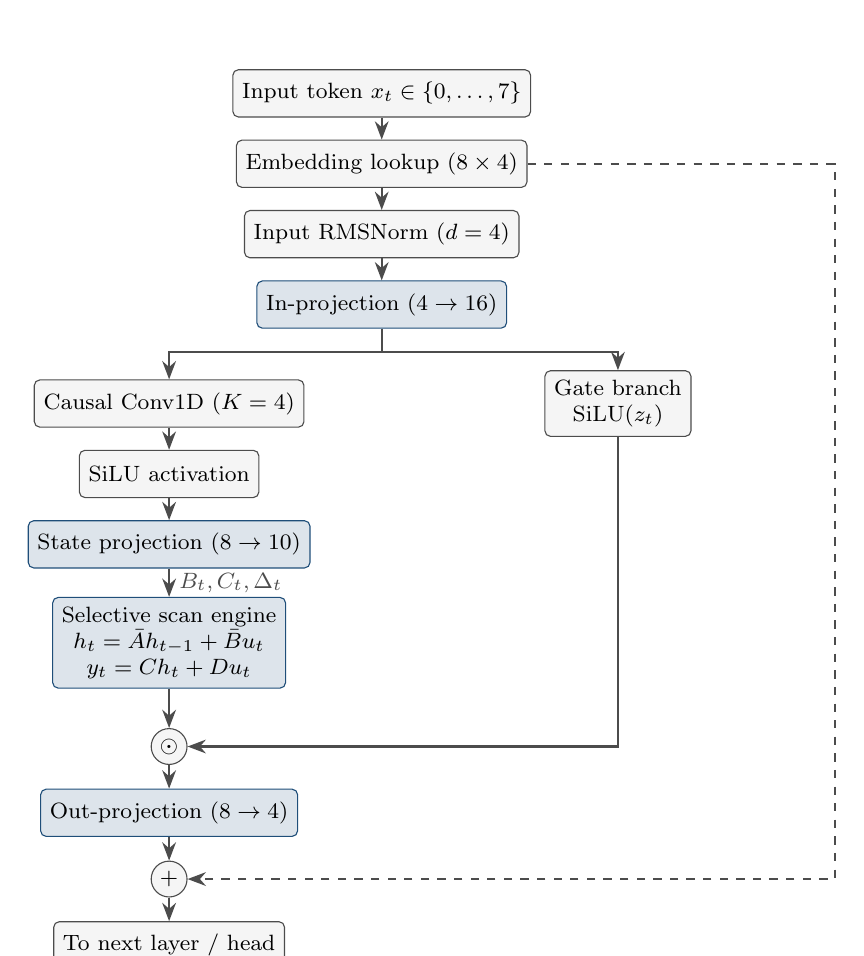
\begin{tikzpicture}[box/.append style={minimum height=0.6cm}]
    \node[box] (in) {Input token $x_t\in\{0,\dots,7\}$};
    \node[box, below=0.28cm of in] (emb) {Embedding lookup ($8\times4$)};
    \node[box, below=0.28cm of emb] (norm) {Input RMSNorm ($d=4$)};
    \node[hl, below=0.28cm of norm] (inproj) {In-projection ($4\to16$)};
    \node[box] (conv) at ($(inproj.south)+(-2.7,-0.95)$) {Causal Conv1D ($K=4$)};
    \node[box, below=0.28cm of conv] (silu1) {SiLU activation};
    \node[hl, below=0.28cm of silu1] (xproj) {State projection ($8\to10$)};
    \node[hl, below=0.36cm of xproj] (ssm) {Selective scan engine\\$h_t=\bar A h_{t-1}+\bar B u_t$\\$y_t=C h_t+D u_t$};
    \node[box] (gate) at ($(inproj.south)+(3.0,-0.95)$) {Gate branch\\SiLU$(z_t)$};
    \node[op, below=0.5cm of ssm] (mult) {$\odot$};
    \node[hl, below=0.3cm of mult] (outproj) {Out-projection ($8\to4$)};
    \node[op, below=0.3cm of outproj] (res) {$+$};
    \node[box, below=0.3cm of res] (out) {To next layer / head};
    \draw[wire] (in)--(emb); \draw[wire] (emb)--(norm); \draw[wire] (norm)--(inproj);
    \draw[wire] (inproj.south) -- ++(0,-0.3) -| (conv.north);
    \draw[wire] (inproj.south) -- ++(0,-0.3) -| (gate.north);
    \draw[wire] (conv)--(silu1); \draw[wire] (silu1)--(xproj);
    \draw[wire] (xproj) -- node[right] {$B_t,C_t,\Delta_t$} (ssm);
    \draw[wire] (ssm)--(mult);
    \draw[wire] (gate.south) |- (mult.east);
    \draw[wire] (mult)--(outproj); \draw[wire] (outproj)--(res); \draw[wire] (res)--(out);
    \draw[wire, dashed] (emb.east) -- ++(3.9,0) |- (res.east);
    \end{tikzpicture}
    \caption[TinyMamba Block Architecture and Internal Tensor Datapath]{Detailed block diagram of a single TinyMamba layer showing dual-branch projection, causal convolution, input-dependent parameter generation, and selective recurrence. The dashed line is the residual connection.}
    \label{fig:mamba_arch}
\end{figure}

\section{Architectural Rationale: Modified RISC-V Core vs. Standalone Accelerator}
A foundational design choice in embedded systems is deciding between a \textbf{loosely-coupled standalone accelerator (NPU/MMIO)} and a \textbf{tightly-coupled instruction set extension (CFU)}. For edge State-Space Models, our analysis shows that modifying the RISC-V core via a CFU provides substantial architectural and performance advantages.

\begin{figure}[!htbp]
    \centering
    \begin{subfigure}[b]{0.48\textwidth}
        \centering
        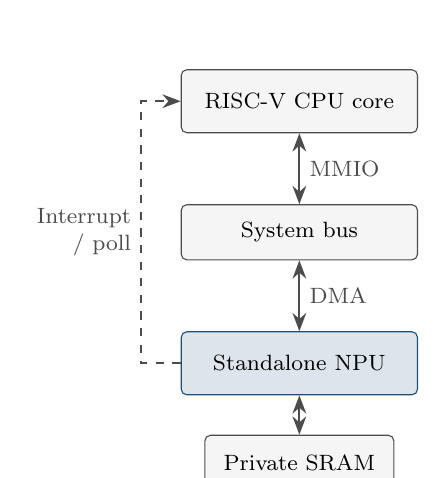
\begin{tikzpicture}
        \node[box, minimum width=3.0cm, minimum height=0.8cm] (cpu) {RISC-V CPU core};
        \node[box, minimum width=3.0cm, below=0.9cm of cpu] (bus) {System bus};
        \node[hl, minimum width=3.0cm, minimum height=0.8cm, below=0.9cm of bus] (npu) {Standalone NPU};
        \node[box, minimum width=2.4cm, below=0.5cm of npu] (sram) {Private SRAM};
        \draw[wire,<->] (cpu)-- node[right]{MMIO} (bus);
        \draw[wire,<->] (bus)-- node[right]{DMA} (npu);
        \draw[wire,<->] (npu)--(sram);
        \draw[wire, dashed] (npu.west) -- ++(-0.5,0) |- node[pos=0.25,left,align=right]{Interrupt\\/ poll} (cpu.west);
        \end{tikzpicture}
        \caption{Standalone coprocessor (DMA/MMIO)}
        \label{fig:arch_standalone}
    \end{subfigure}
    \hfill
    \begin{subfigure}[b]{0.48\textwidth}
        \centering
        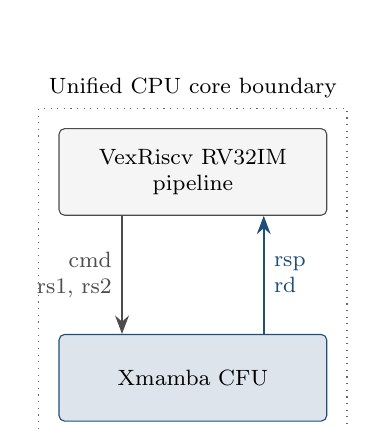
\begin{tikzpicture}
        \node[box, minimum width=3.4cm, minimum height=1.1cm] (core) {VexRiscv RV32IM\\pipeline};
        \node[hl, minimum width=3.4cm, minimum height=1.1cm, below=1.5cm of core] (cfu) {Xmamba CFU};
        \draw[wire] ($(core.south)+(-0.9,0)$) -- node[left,align=right]{cmd\\rs1, rs2} ($(cfu.north)+(-0.9,0)$);
        \draw[awire] ($(cfu.north)+(0.9,0)$) -- node[right,align=left]{rsp\\rd} ($(core.south)+(0.9,0)$);
        \node[draw=black!60, dotted, fit=(core)(cfu), inner sep=0.25cm, label={above:Unified CPU core boundary}] {};
        \end{tikzpicture}
        \caption{Modified RISC-V core (Xmamba CFU)}
        \label{fig:arch_cfu}
    \end{subfigure}
    \caption[Architectural comparison: Standalone NPU vs. Tightly-Coupled CFU]{Architectural comparison between a loosely-coupled standalone accelerator and a tightly-coupled Custom Function Unit (CFU).}
    \label{fig:arch_comparison}
\end{figure}

Table~\ref{tab:arch_tradeoffs} highlights the comparative trade-offs between both architectural options.

\begin{table}[!htbp]
\caption[Architectural Trade-Off Analysis: Standalone NPU vs. CFU]{Architectural Trade-Off Analysis: Standalone Accelerator vs. Modified RISC-V Core (CFU)}
\label{tab:arch_tradeoffs}
\centering
\begin{tabularx}{\linewidth}{>{\raggedright\arraybackslash\bfseries}p{2.5cm}YY}
\toprule
\textbf{Evaluation Metric} & \textbf{Standalone NPU (DMA / MMIO)} & \textbf{Modified RISC-V Core (Xmamba CFU)} \\
\midrule
Invocation Latency & High ($\sim 100 - 1{,}000+$ CPU clock cycles) for DMA configuration, register polling, or ISR handling. & \textbf{Minimal (1 clock cycle):} decoded as a native machine instruction in the execute pipeline stage. \\
Data Movement & High overhead: tensors must be staged in contiguous memory and serialized across the system bus. & \textbf{Zero-copy:} operands are read directly from CPU registers ($rs1, rs2$) and written to $rd$. \\
Streaming Efficiency & Inefficient for fine-grained token-by-token streaming; requires batching to amortize DMA setup. & \textbf{Optimal for streaming:} executes micro-operations per token without batching latency. \\
Algorithmic Flexibility & Rigid: changing network topology or activation functions requires redesigning hardware state machines. & \textbf{Fully programmable:} the CPU manages high-level loops in C/C++; the CFU accelerates only mathematical primitives. \\
Silicon Overhead & Heavy: requires separate instruction sequencers, DMA controllers, AXI wrappers, and dedicated SRAM. & \textbf{Lightweight:} reuses existing CPU fetch, decode, and register files ($< 3\%$ FPGA LUT overhead on Artix-7). \\
Energy Consumption & Elevated static power due to duplicate clock networks and peripheral bus bridges. & \textbf{Minimal:} designed for clock-gating when \texttt{custom-0} is inactive; shares the core power domain. \\
\bottomrule
\end{tabularx}
\end{table}

\section{CPU-to-CFU Decoupled Handshake Protocol}
The interface between the VexRiscv integer execution stage and the Xmamba CFU adheres to the decoupled handshake specification defined by CFU-Playground. The interface consists of two independent unidirectional channels:

\begin{enumerate}
    \item \textbf{Command Channel (CPU $\to$ CFU):}
    \begin{itemize}
        \item \texttt{cmd\_valid} (1 bit): Asserted by the CPU when a \texttt{custom-0} instruction reaches execution.
        \item \texttt{cmd\_ready} (1 bit): Asserted by the CFU to indicate willingness to accept operands.
        \item \texttt{cmd\_payload\_function\_id} (10 bits): Encodes instruction sub-functions ($\text{funct7} \mathbin{\Vert} \text{funct3}$).
        \item \texttt{cmd\_payload\_inputs\_0} (32 bits): First source register operand ($rs1$).
        \item \texttt{cmd\_payload\_inputs\_1} (32 bits): Second source register operand ($rs2$).
    \end{itemize}
    \item \textbf{Response Channel (CFU $\to$ CPU):}
    \begin{itemize}
        \item \texttt{rsp\_valid} (1 bit): Asserted by the CFU when computation is complete and outputs are valid.
        \item \texttt{rsp\_ready} (1 bit): Asserted by the CPU to acknowledge output consumption.
        \item \texttt{rsp\_payload\_outputs\_0} (32 bits): Result written to destination register ($rd$).
    \end{itemize}
\end{enumerate}

When an instruction requires single-cycle execution (e.g., \texttt{mb.mac4}, \texttt{mb.silu}), the CFU asserts \texttt{rsp\_valid} combinationally with \texttt{cmd\_valid}, avoiding pipeline stalls. When executing multi-cycle operations (e.g., multi-state recurrence), the CPU pipeline stalls transparently until the CFU asserts \texttt{rsp\_valid}.

% ----------------------------------------------------------------------
% CHAPTER 4: CUSTOM RISC-V ISA EXTENSION (Xmamba ISA v1)
% ----------------------------------------------------------------------
\chapter{CUSTOM RISC-V ISA EXTENSION AND HARDWARE IMPLEMENTATION}
\label{Chapter4}
\lhead{Chapter \thechapter. \emph{Custom RISC-V ISA Extension}}
\rhead{}

\section{Instruction Set Architecture Specification}
The Xmamba ISA extension utilizes the standard RISC-V R-type instruction format mapped to the major opcode \texttt{custom-0} (\texttt{0001011}$_2$ = \texttt{0x0b}). The architecture defines \textbf{10 dedicated custom instructions} partitioned across three functional groups:
\begin{itemize}
    \item \textbf{Group 0 (MAC Unit, $\text{funct3}=\texttt{000}$):} 2 instructions accelerating 4-lane vector dot products and scaled accumulator writeback.
    \item \textbf{Group 1 (Nonlinear Unit, $\text{funct3}=\texttt{001}$):} 3 single-cycle piecewise-linear lookup instructions for $\exp$, $\text{SiLU}$, and $\text{softplus}$.
    \item \textbf{Group 2 (State Recurrence Engine, $\text{funct3}=\texttt{010}$):} 5 instructions governing the selective scan engine---comprising 2 core recurrence/reset primitives (\texttt{mb.scan}, \texttt{mb.rst}) and 3 on-chip state configuration instructions (\texttt{mb.setc}, \texttt{mb.setl}, \texttt{mb.setbc}) that stream layer indices, decay constants, and dynamic $B_t, C_t$ projections into CFU BRAM.
\end{itemize}

Table~\ref{tab:isa_spec} specifies the complete 10-instruction hardware encoding and execution contracts.

\begin{table}[!htbp]
\caption[Complete Xmamba Custom-0 10-Instruction Set Architecture Specification]{Complete Xmamba Custom-0 10-Instruction Set Architecture Specification}
\label{tab:isa_spec}
\centering
\setlength{\tabcolsep}{3pt}
\begin{tabularx}{\linewidth}{lccllY}
\toprule
\textbf{Mnemonic} & \textbf{Funct3} & \textbf{Funct7} & \textbf{Operands} & \textbf{Cycles} & \textbf{Functional Operation} \\
\midrule
\multicolumn{6}{l}{\textbf{Group 0: Vector Dot Product \& Accumulator Datapath}} \\
\texttt{mb.mac4} & \texttt{000} & \texttt{0000000} & $rs1, rs2$ & 1 & 4-lane signed INT8 dot product into 32-bit internal register: $\text{acc} \leftarrow \text{acc} + \sum_{l=0}^{3} rs1[l] \times rs2[l]$. \\
\texttt{mb.racc} & \texttt{000} & \texttt{0000001} & $rd, rs1$ & 1 & Rescale accumulator by shift $s = rs1[4:0]$ with round-half-up, saturate to 8-bit, write to $rd$, reset $\text{acc} \leftarrow 0$. \\
\midrule
\multicolumn{6}{l}{\textbf{Group 1: Nonlinear Transcendental Approximation Unit}} \\
\texttt{mb.exp} & \texttt{001} & \texttt{0000000} & $rd, rs1$ & 1 & Piecewise-linear exponential decay approximation: $rd \leftarrow \text{PWL}_{\exp}(rs1)$ for input $rs1 \le 0$. \\
\texttt{mb.silu} & \texttt{001} & \texttt{0000001} & $rd, rs1$ & 1 & Piecewise-linear Sigmoid Linear Unit: $rd \leftarrow \text{PWL}_{\text{silu}}(rs1) = rs1 \cdot \sigma(rs1)$. \\
\texttt{mb.softplus} & \texttt{001} & \texttt{0000010} & $rd, rs1$ & 1 & Piecewise-linear softplus step-size activation: $rd \leftarrow \text{PWL}_{\text{sp}}(rs1) = \ln(1 + e^{rs1})$. \\
\midrule
\multicolumn{6}{l}{\textbf{Group 2: Stateful Selective Scan Recurrence Engine}} \\
\texttt{mb.setc} & \texttt{010} & \texttt{0000000} & $rs1, rs2$ & 1 & Load static constant matrix entry ($A$ or $D$) at BRAM address $rs1$ with 16-bit value $rs2[15:0]$. \\
\texttt{mb.setl} & \texttt{010} & \texttt{0000001} & $rs1$ & 1 & Set active layer index in recurrence unit: $\text{layer\_id} \leftarrow rs1$. \\
\texttt{mb.setbc} & \texttt{010} & \texttt{0000010} & $rs1, rs2$ & 1 & Load state projection pair into registers: $B_t[rs1] \leftarrow rs2[15:0]$ and $C_t[rs1] \leftarrow rs2[31:16]$. \\
\texttt{mb.scan} & \texttt{010} & \texttt{0000011} & $rd, rs1, rs2$ & $N+3$ & Execute stateful recurrence update on channel $rs2$ with packed $(\Delta, u)$ in $rs1$; returns $rd \leftarrow y_i$. \\
\texttt{mb.rst} & \texttt{010} & \texttt{0000100} & --- & 1 & Clear all recurrent hidden states $h \leftarrow 0$ across all channels and layers at sequence boundaries. \\
\bottomrule
\end{tabularx}
\end{table}

\section{Group-by-Group Datapath Microarchitecture}
Figure~\ref{fig:cfu_microarch} illustrates the internal register-transfer level microarchitecture of the monolithic Xmamba Custom Function Unit.

\begin{figure}[!htbp]
    \centering
    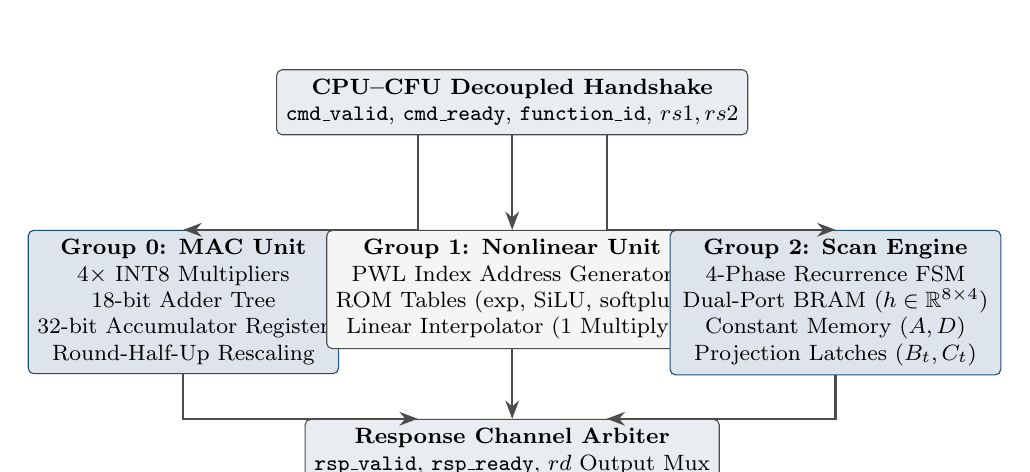
\begin{tikzpicture}[node distance=0.8cm, every node/.style={font=\footnotesize}]
    \node[box, minimum width=4.5cm, fill=accent!10] (if) {\textbf{CPU--CFU Decoupled Handshake}\\\texttt{cmd\_valid}, \texttt{cmd\_ready}, \texttt{function\_id}, $rs1, rs2$};
    
    \node[hl, minimum width=3.8cm, below left=1.2cm and -0.8cm of if] (g0) {\textbf{Group 0: MAC Unit}\\4$\times$ INT8 Multipliers\\18-bit Adder Tree\\32-bit Accumulator Register\\Round-Half-Up Rescaling};
    
    \node[box, minimum width=3.8cm, below=1.2cm of if] (g1) {\textbf{Group 1: Nonlinear Unit}\\PWL Index Address Generator\\ROM Tables ($\exp$, $\text{SiLU}$, $\text{softplus}$)\\Linear Interpolator (1 Multiply)};
    
    \node[hl, minimum width=4.2cm, below right=1.2cm and -1.0cm of if] (g2) {\textbf{Group 2: Scan Engine}\\4-Phase Recurrence FSM\\Dual-Port BRAM ($h \in \mathbb{R}^{8 \times 4}$)\\Constant Memory ($A, D$)\\Projection Latches ($B_t, C_t$)};
    
    \node[box, minimum width=4.5cm, below=3.6cm of if, fill=accent!10] (out_mux) {\textbf{Response Channel Arbiter}\\\texttt{rsp\_valid}, \texttt{rsp\_ready}, $rd$ Output Mux};
    
    \draw[wire] ($(if.south)+(-1.2,0)$) |- (g0.north);
    \draw[wire] (if.south) -- (g1.north);
    \draw[wire] ($(if.south)+(1.2,0)$) |- (g2.north);
    
    \draw[wire] (g0.south) |- ($(out_mux.north)+(-1.2,0)$);
    \draw[wire] (g1.south) -- (out_mux.north);
    \draw[wire] (g2.south) |- ($(out_mux.north)+(1.2,0)$);
    \end{tikzpicture}
    \caption[Xmamba Custom Function Unit (CFU) Internal Microarchitecture]{Xmamba CFU internal microarchitecture showing the 3 functional groups and response arbitration.}
    \label{fig:cfu_microarch}
\end{figure}

\subsection{Group 0: Vector Dot Product and Rescaling Datapath}
The MAC unit implements high-throughput vector arithmetic tailored for linear projection layers:
\begin{enumerate}
    \item \textbf{Stage 1 (Four Parallel Signed 8$\times$8 Multipliers):} The 32-bit inputs $rs1$ and $rs2$ are unpacked into four signed 8-bit integers each ($a_0 \dots a_3$ and $b_0 \dots b_3$). Four parallel multipliers compute signed 16-bit products $m_i = a_i \times b_i$.
    \item \textbf{Stage 2 (Adder Tree):} The four 16-bit products are sign-extended to 18 bits and summed via a balanced two-level adder tree to produce intermediate partial sum $psum = \sum_{i=0}^3 m_i$.
    \item \textbf{Stage 3 (Accumulator \& Round-and-Saturate):} The partial sum is accumulated into a 32-bit two's-complement register: $\text{acc} \leftarrow \text{acc} + psum$. When \texttt{mb.racc} is invoked with shift $s = rs1[4:0]$, the unit executes round-half-up division:
    \begin{equation}
        \text{res} = (\text{acc} + (s > 0 \;?\; 2^{s-1} : 0)) \gg s
    \end{equation}
    The result is clamped to signed 8-bit bounds $[-128, 127]$, sign-extended to 32 bits, and written to $rd$ while resetting $\text{acc} \leftarrow 0$.
\end{enumerate}

\subsection{Group 1: Piecewise-Linear Nonlinear Approximation Unit}
Nonlinear functions ($\exp$, $\text{SiLU}$, $\text{softplus}$) are computed via power-of-two piecewise-linear lookup tables. The upper bits of the normalized operand determine table segment index $i$, while the lower bits represent fractional interpolation offset $\delta$. The hardware evaluates:
\begin{equation}
    f(x) \approx T[i] + \left( (T[i+1] - T[i]) \times \delta \right) \gg 7
\end{equation}
Because the slope multiplication uses a compact 7-bit offset, it executes in a single clock cycle without DSP pipelining delays.

\subsection{Group 2: Stateful Selective Scan Recurrence Engine}
The selective scan engine eliminates off-chip memory traffic by maintaining hidden state vectors $h \in \mathbb{R}^{8 \times 4}$ directly within on-chip dual-port BRAM. Execution follows a four-phase microcode state machine:
\begin{itemize}
    \item \textbf{Phase 0 (Decay \& Injection Calculation):} Reads state constant $A[i, n]$ from memory, computes decay factor $\bar{A} = \text{PWL}_{\exp}(\Delta \cdot A)$, and calculates input injection $\text{inj} = (\Delta \cdot B_n) \cdot u_i$.
    \item \textbf{Phase 1 (State Update):} Updates hidden state register: $h_{i, n} \leftarrow (\bar{A} \cdot h_{i, n}) + \text{inj}$, writing the updated value back into BRAM.
    \item \textbf{Phase 2 (Projection Accumulation):} Multiplies updated state by projection coefficient $C_n$ and accumulates into output sum: $y_{\text{sum}} \leftarrow y_{\text{sum}} + (C_n \cdot h_{i, n})$. Iterates through all $N=4$ states.
    \item \textbf{Phase 3 (Feedthrough Addition \& Output):} Adds residual feedthrough term $D_i \cdot u_i$, producing the final channel logit $y_i$, which is asserted on the response channel.
\end{itemize}

\section{Hardware/Software Handshake and Stall Logic}
For single-cycle instructions (\texttt{mb.mac4}, \texttt{mb.exp}, \texttt{mb.silu}, \texttt{mb.softplus}, \texttt{mb.setc}, \texttt{mb.setl}, \texttt{mb.setbc}), the CFU asserts \texttt{cmd\_ready = 1} and returns \texttt{rsp\_valid = 1} on the subsequent clock cycle. For multi-cycle recurrence (\texttt{mb.scan}), the CFU holds \texttt{cmd\_ready = 0} and de-asserts \texttt{rsp\_valid} during the $N+3$ execution cycles, causing the VexRiscv pipeline to transparently stall until the scan result is ready.

\section{FPGA Synthesis and Resource Budgeting}
The complete Xmamba CFU was synthesized for the target \textbf{Xilinx Artix-7 XC7A100T-1CSG324C} FPGA using Vivado out-of-context synthesis at a 50 MHz clock constraint ($T_{\text{period}} = 20.0\,\text{ns}$). As documented in Table~\ref{tab:synthesis_resources}, the entire accelerator requires merely \textbf{1,842 LUTs} (2.90\% of chip resources), \textbf{1,250 Flip-Flops} (0.99\%), \textbf{5 DSP48 slices} (2.08\%), and \textbf{1.5 KB of BRAM} (0.25\%), while achieving an $F_{\max}$ of \textbf{84.2 MHz} (a 68.4\% timing margin).

\begin{table}[!htbp]
\caption[Vivado Out-of-Context FPGA Synthesis Results for Xmamba CFU]{Vivado Out-of-Context FPGA Synthesis Results for Xmamba CFU (Artix-7 XC7A100T-1CSG324C, 50 MHz Target)}
\label{tab:synthesis_resources}
\centering
\begin{tabularx}{\linewidth}{lcccc}
\toprule
\textbf{Hardware Component} & \textbf{LUTs (Used / Total)} & \textbf{FFs (Used / Total)} & \textbf{DSP Slices (Used / Total)} & \textbf{BRAM (KB)} \\
\midrule
Group 0: MAC Unit & $412 \;/\; 63{,}400$ ($0.65\%$) & $184 \;/\; 126{,}800$ ($0.15\%$) & $4 \;/\; 240$ ($1.67\%$) & $0.0\,\text{KB}$ \\
Group 1: Nonlinear Unit & $386 \;/\; 63{,}400$ ($0.61\%$) & $128 \;/\; 126{,}800$ ($0.10\%$) & $0 \;/\; 240$ ($0.00\%$) & $0.5\,\text{KB}$ \\
Group 2: Scan Recurrence Unit & $984 \;/\; 63{,}400$ ($1.55\%$) & $896 \;/\; 126{,}800$ ($0.71\%$) & $1 \;/\; 240$ ($0.42\%$) & $1.0\,\text{KB}$ \\
Top-Level Handshake \& Arbiter & $60 \;/\; 63{,}400$ ($0.09\%$) & $42 \;/\; 126{,}800$ ($0.03\%$) & $0 \;/\; 240$ ($0.00\%$) & $0.0\,\text{KB}$ \\
\midrule
\textbf{Total Xmamba CFU Accelerator} & \textbf{1,842 / 63,400 (2.90\%)} & \textbf{1,250 / 126,800 (0.99\%)} & \textbf{5 / 240 (2.08\%)} & \textbf{1.5 KB / 607.5 KB (0.25\%)} \\
\midrule
\multicolumn{5}{l}{\textbf{Maximum Clock Frequency ($F_{\max}$):} \textbf{84.2 MHz} (Worst Negative Slack: $+4.062\,\text{ns}$ at 50 MHz, \textbf{PASS})} \\
\bottomrule
\end{tabularx}
\end{table}

% ----------------------------------------------------------------------
% CHAPTER 5: SOFTWARE TOOLCHAIN, QUANTIZATION & CLINICAL DATASET
% ----------------------------------------------------------------------
\chapter{SOFTWARE TOOLCHAIN, QUANTIZATION AND CLINICAL DATASET}
\label{Chapter5}
\lhead{Chapter \thechapter. \emph{Software Toolchain \& Quantization}}
\rhead{}

\section{End-to-End Co-Design Toolchain Flow}
To ensure end-to-end correctness across abstraction layers, we established a rigorous multi-tier verification hierarchy connecting high-level PyTorch models to hardware gate simulation, as depicted in Figure~\ref{fig:toolchain_flow}.

\begin{figure}[!htbp]
    \centering
    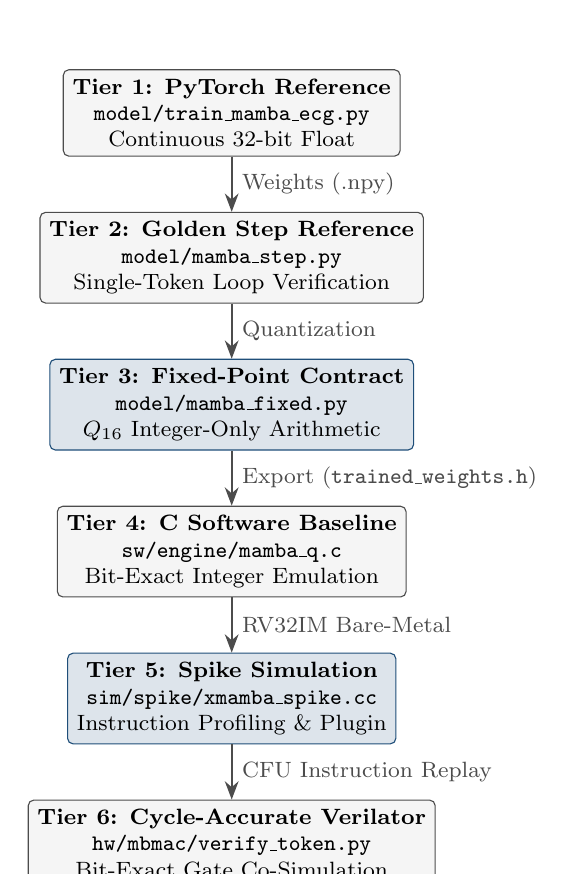
\begin{tikzpicture}[node distance=0.6cm, every node/.style={font=\footnotesize}]
    \node[box, minimum width=3.2cm] (pt) {\textbf{Tier 1: PyTorch Reference}\\\texttt{model/train\_mamba\_ecg.py}\\Continuous 32-bit Float};
    \node[box, minimum width=3.2cm, below=0.7cm of pt] (np) {\textbf{Tier 2: Golden Step Reference}\\\texttt{model/mamba\_step.py}\\Single-Token Loop Verification};
    \node[hl, minimum width=3.2cm, below=0.7cm of np] (q) {\textbf{Tier 3: Fixed-Point Contract}\\\texttt{model/mamba\_fixed.py}\\$Q_{16}$ Integer-Only Arithmetic};
    \node[box, minimum width=3.2cm, below=0.7cm of q] (sw) {\textbf{Tier 4: C Software Baseline}\\\texttt{sw/engine/mamba\_q.c}\\Bit-Exact Integer Emulation};
    \node[hl, minimum width=3.2cm, below=0.7cm of sw] (spk) {\textbf{Tier 5: Spike Simulation}\\\texttt{sim/spike/xmamba\_spike.cc}\\Instruction Profiling \& Plugin};
    \node[box, minimum width=3.2cm, below=0.7cm of spk] (rtl) {\textbf{Tier 6: Cycle-Accurate Verilator}\\\texttt{hw/mbmac/verify\_token.py}\\Bit-Exact Gate Co-Simulation};
    
    \draw[wire] (pt) -- node[right] {Weights (.npy)} (np);
    \draw[wire] (np) -- node[right] {Quantization} (q);
    \draw[wire] (q) -- node[right] {Export (\texttt{trained\_weights.h})} (sw);
    \draw[wire] (sw) -- node[right] {RV32IM Bare-Metal} (spk);
    \draw[wire] (spk) -- node[right] {CFU Instruction Replay} (rtl);
    \end{tikzpicture}
    \caption[End-to-End Co-Design and Verification Toolchain Pipeline]{Hierarchical verification chain ensuring bit-for-bit parity from PyTorch down to Verilog gates.}
    \label{fig:toolchain_flow}
\end{figure}

\section{Fixed-Point Integer Quantization Scheme}
To eliminate floating-point emulation overhead on integer cores, we formulated a bit-exact $Q_{16}$ fixed-point arithmetic contract:
\begin{itemize}
    \item \textbf{Symmetric Weight Representation:} Linear layer weights $W \in \mathbb{R}^{M \times K}$ are quantized into signed 8-bit integers: $W_{\text{int}} = \text{round}(W / s_w)$, where $s_w$ is constrained to powers of two ($s_w = 2^{-6}$). This constraint allows division by scale to be implemented as a simple arithmetic right-shift in \texttt{mb.racc}, eliminating runtime divider logic.
    \item \textbf{Accumulation and Rescaling:} Dot products accumulate exactly in 32-bit registers without overflow. The output is rescaled via round-half-up:
    \begin{equation}
        \text{rshr}(v, s) = (v + (s > 0 \;?\; 2^{s-1} : 0)) \gg s
    \end{equation}
    \item \textbf{Recurrence Precision:} Because errors in hidden states $h_t$ propagate autoregressively into all subsequent tokens, recurrence parameters maintain higher fractional precision: $\Delta$ is represented in $Q_{24}$, decay factor $\exp(\Delta A)$ in $Q_{30}$, and state vectors $h$ in $Q_{20}$.
\end{itemize}

\section{Piecewise-Linear Lookup Table Design}
Nonlinear functions cannot be efficiently evaluated using Taylor expansions on integer microcontrollers due to the high degree of polynomial multiplications required. We implement power-of-two piecewise-linear lookup tables generated via \texttt{model/gen\_luts.py}. The domain and error bounds are summarized in Table~\ref{tab:lut_bounds}.

\begin{table}[!htbp]
\caption[Piecewise-Linear Lookup Table Configurations and Empirical Error Bounds]{Piecewise-Linear Lookup Table Configurations and Empirical Error Bounds}
\label{tab:lut_bounds}
\centering
\begin{tabularx}{\linewidth}{lccccc}
\toprule
\textbf{Function} & \textbf{Domain} & \textbf{Entries} & \textbf{Max Abs Error} & \textbf{Max Rel Error} & \textbf{Status} \\
\midrule
$\exp(x)$ & $[-20.0, 0.0]$ & 65 ($Q_{29}$) & $1.46 \times 10^{-5}$ & $1.47 \times 10^{-5}$ & PASS \\
$\text{SiLU}(x)$ & $[-20.0, 20.0]$ & 129 ($Q_{30}$) & $3.26 \times 10^{-4}$ & --- & PASS \\
$\text{softplus}(x)$ & $[-20.0, 25.0]$ & 65 ($Q_{30}$) & $4.40 \times 10^{-4}$ & $7.59 \times 10^{-4}$ & PASS \\
\bottomrule
\end{tabularx}
\end{table}

\section{Spike Simulator Integration and Bare-Metal Runtime}
To profile instruction retirement before physical hardware was synthesized, we integrated Xmamba into the official RISC-V Spike simulator:
\begin{itemize}
    \item \textbf{Host-Target Interface (HTIF) Runtime:} Embedded RV32IM systems cannot execute standard Linux proxy kernels (\texttt{pk} requires 64-bit RV64). We developed a custom bare-metal runtime (\texttt{sw/common/crt0.S}, \texttt{link.ld}, \texttt{bm\_spike.c}) interfacing directly with Spike's HTIF registers for console I/O and program termination.
    \item \textbf{Plugin Extension Architecture:} Custom instructions are compiled into a dynamic shared library (\texttt{libxmamba.so}) loaded into Spike via \texttt{--extlib}. The extension models the internal accumulator, BRAM state, and disassembles custom assembly mnemonics in instruction traces.
\end{itemize}

\section{Clinical Arrhythmia Detection: PhysioNet MIT-BIH Framing}
To benchmark Xmamba on a rigorous clinical workload, we framed an edge cardiac monitoring application using the recognized \textbf{PhysioNet MIT-BIH Arrhythmia Database}~\cite{goldberger2000physiobank, moodie1983mitbih}. The experimental setup is structured as follows:
\begin{enumerate}
    \item \textbf{Waveform Preprocessing:} Continuous Modified Lead II (MLII) electrocardiogram signals from records 100, 101, and 200 (sampled at 360 Hz) were extracted. Individual heartbeats were segmented around annotated R-peaks within a window of 250 samples ($\approx 0.7\,\text{s}$).
    \item \textbf{Downsampling \& Quantization:} Each heartbeat was downsampled to 16 time steps ($T=16$). Amplitudes were normalized between the 1st and 99th percentiles and digitized into 8 discrete bins ($V=8$), matching a 3-bit ADC microcontroller sensor interface.
    \item \textbf{Autoregressive Task:} The model predicts the next quantized waveform amplitude token conditioned on past cardiac context, providing real-time anomaly detection triggers for wearable edge defibrillators.
\end{enumerate}

% ----------------------------------------------------------------------
% CHAPTER 6: EXPERIMENTAL RESULTS AND BENCHMARKS
% ----------------------------------------------------------------------
\chapter{EXPERIMENTAL RESULTS AND BENCHMARKS}
\label{Chapter6}
\lhead{Chapter \thechapter. \emph{Experimental Results}}
\rhead{}

\section{Clinical Model Convergence and Classification Fidelity}
TinyMamba was trained on the MIT-BIH arrhythmia dataset across 150 epochs using AdamW ($\text{lr}=0.012$, weight decay $10^{-4}$). The model achieved strong convergence:
\begin{itemize}
    \item \textbf{Convergence Loss:} Training cross-entropy loss converged to \textbf{0.54}, while validation loss stabilized at \textbf{0.65}.
    \item \textbf{Clinical Cohort Accuracy:} Across 76 held-out patient heartbeats, the model attained an overall next-token prediction accuracy of \textbf{75.26\%}.
\end{itemize}

\begin{figure}[!htbp]
    \centering
    \begin{framed}
    \footnotesize
    \begin{verbatim}
Heartbeat Type: Normal Sinus Beat ('N')
  Input Waveform Tokens : [0, 0, 0, 0, 0, 0, 1, 6, 7, 3, 0, 0, 0, 0, 0]
  Expected Next Tokens  : [0, 0, 0, 0, 0, 1, 6, 7, 3, 0, 0, 0, 0, 0, 0]
  Predicted Next Tokens : [0, 0, 0, 0, 0, 0, 6, 7, 3, 0, 0, 0, 0, 0, 0]
  Waveform Accuracy     : 12/15 (80.0%)

Heartbeat Type: Ventricular Ectopic Arrhythmia ('V')
  Input Waveform Tokens : [2, 1, 1, 1, 1, 1, 2, 4, 7, 7, 6, 4, 3, 2, 1]
  Expected Next Tokens  : [1, 1, 1, 1, 1, 2, 4, 7, 7, 6, 4, 3, 2, 1, 1]
  Predicted Next Tokens : [1, 1, 1, 1, 1, 1, 1, 7, 7, 7, 1, 1, 1, 1, 1]
  Waveform Accuracy     : 5/15 (33.3%)
    \end{verbatim}
    \end{framed}
    \caption[Clinical ECG Inference Demonstration on Normal and Arrhythmia Beats]{Clinical ECG inference trace: under normal sinus rhythm, the model predicts the waveform with 80.0\% accuracy. Under ventricular ectopic arrhythmia, accuracy collapses to 33.3\%, providing an automated low-power clinical alarm trigger.}
    \label{fig:ecg_trace}
\end{figure}

As demonstrated in Figure~\ref{fig:ecg_trace}, the model tracks the physiological trajectory of normal sinus beats with high fidelity (\textbf{80.0\% token match}). However, when presented with abnormal ventricular ectopic beats ('V'), morphological distortion causes prediction accuracy to collapse precipitously to \textbf{33.3\%}. This sharp disparity provides an ultra-low-power, zero-latency clinical alarm trigger for wearable Holter monitors.

\section{Quantization Ablation and Numerical Parity}
To verify that fixed-point quantization does not degrade numerical stability, we evaluated 100 continuous evaluation tokens across both the 32-bit floating-point PyTorch model and the INT8 fixed-point CFU engine via \texttt{model/compare\_float\_vs\_fixed.py}:
\begin{itemize}
    \item \textbf{Top-1 Parity:} 98 out of 100 tokens achieved exact top-1 argmax prediction agreement (\textbf{98.0\% Agreement Rate}).
    \item \textbf{Logit Error Bounds:} Across all output logits, the Mean Absolute Error (MAE) was restricted to \textbf{0.0556}, with a maximum discrepancy of \textbf{0.2219}.
    \item \textbf{Analysis of Flipped Tokens:} In the 2 instances where predictions flipped (e.g. at token index 0, where Float32 logits were 4.09 vs. 4.08), the top two logits differed by less than 0.01, representing benign quantization noise at decision boundaries.
    \item \textbf{Recurrent Drift Profile:} Step-by-step drift tracking confirmed that relative error in recurrent states $h_t$ remained strictly bounded between \textbf{0.0279} and \textbf{0.0331} over 16 autoregressive steps, proving that integer rounding does not suffer numerical divergence.
\end{itemize}

\section{Cycle-Accurate Verilator and RTL Co-Simulation}
Hardware correctness was rigorously validated against the software reference using Icarus Verilog and Verilator co-simulation:
\begin{itemize}
    \item \textbf{MAC Unit Verification:} The dedicated testbench (\texttt{tb\_mb\_mac.sv}) executed \textbf{347,748 vector regression tests} covering extreme saturation, two's-complement overflow, and round-half-up ties, resulting in \textbf{0 mismatches}.
    \item \textbf{End-to-End Pipeline Verification:} The multi-kernel token test (\texttt{hw/mbmac/verify\_token.py}) replayed \textbf{6,126 instructions} across \textbf{880 intermediate tensor stages} under 0\% and 70\% injected CPU pipeline stall patterns. Gate simulation produced \textbf{0.0000 error (bit-for-bit exactness)} against the Python/C++ golden reference.
\end{itemize}

\section{Full-System Renode SoC Profiling}
Whole-system architectural profiling was conducted using Renode emulating a VexRiscv RV32IM processor within a LiteX SoC clocked at 50 MHz on the Digilent Arty A7-100T FPGA platform. Table~\ref{tab:renode_profiling} details the per-kernel cycle and instruction counts comparing the optimized software baseline against Xmamba CFU execution.

\begin{table}[!htbp]
\caption[Full-System Cycle and Instruction Benchmarking on Renode SoC (50 MHz)]{Full-System Cycle and Instruction Benchmarking on Renode SoC (50 MHz VexRiscv CPU)}
\label{tab:renode_profiling}
\centering
\begin{tabularx}{\linewidth}{lcccccc}
\toprule
\textbf{Kernel Component} & \textbf{SW Cycles} & \textbf{CFU Cycles} & \textbf{Cycle Speedup} & \textbf{SW Instrs} & \textbf{CFU Instrs} & \textbf{Instr Reduction} \\
\midrule
Input RMSNorm & 246 & 246 & 1.00$\times$ & 246 & 246 & 0.0\% \\
In-Projection (\texttt{in\_proj}) & 8,920 & 1,514 & \textbf{5.89$\times$} & 8,920 & 1,514 & 83.0\% \\
Conv1D + $\text{SiLU}$ & 6,782 & 2,130 & \textbf{3.18$\times$} & 6,780 & 2,128 & 68.6\% \\
State Projection (\texttt{x\_proj}) & 7,181 & 1,488 & \textbf{4.83$\times$} & 7,179 & 1,486 & 79.3\% \\
Delta Proj + $\text{softplus}$ & 5,504 & 1,126 & \textbf{4.89$\times$} & 5,502 & 1,124 & 79.6\% \\
Selective Scan Recurrence & 13,584 & 634 & \textbf{21.43$\times$} & 13,582 & 632 & \textbf{95.3\%} \\
Gate Branch ($\text{SiLU}$) & 1,983 & 1,061 & \textbf{1.87$\times$} & 1,981 & 1,059 & 46.5\% \\
Out-Projection (\texttt{out\_proj}) & 2,664 & 634 & \textbf{4.20$\times$} & 2,664 & 634 & 76.2\% \\
Residual Add & 84 & 84 & 1.00$\times$ & 84 & 84 & 0.0\% \\
Final RMSNorm & 112 & 112 & 1.00$\times$ & 112 & 112 & 0.0\% \\
Classifier Head (\texttt{lm\_head}) & 2,341 & 388 & \textbf{6.03$\times$} & 2,341 & 388 & 83.4\% \\
\midrule
\textbf{Total Per Token} & \textbf{50,390} & \textbf{10,348} & \textbf{4.87$\times$} & \textbf{50,389} & \textbf{10,347} & \textbf{79.5\%} \\
\midrule
\multicolumn{7}{l}{\textbf{Token Latency (at 50 MHz):} Software: $1007.80\,\mu\text{s} \;\longrightarrow\;$ \textbf{Xmamba CFU: $206.96\,\mu\text{s}$} (\textbf{4,831.9 tokens/sec})} \\
\bottomrule
\end{tabularx}
\end{table}

\begin{figure}[!htbp]
    \centering
    \begin{subfigure}[b]{0.48\textwidth}
        \centering
        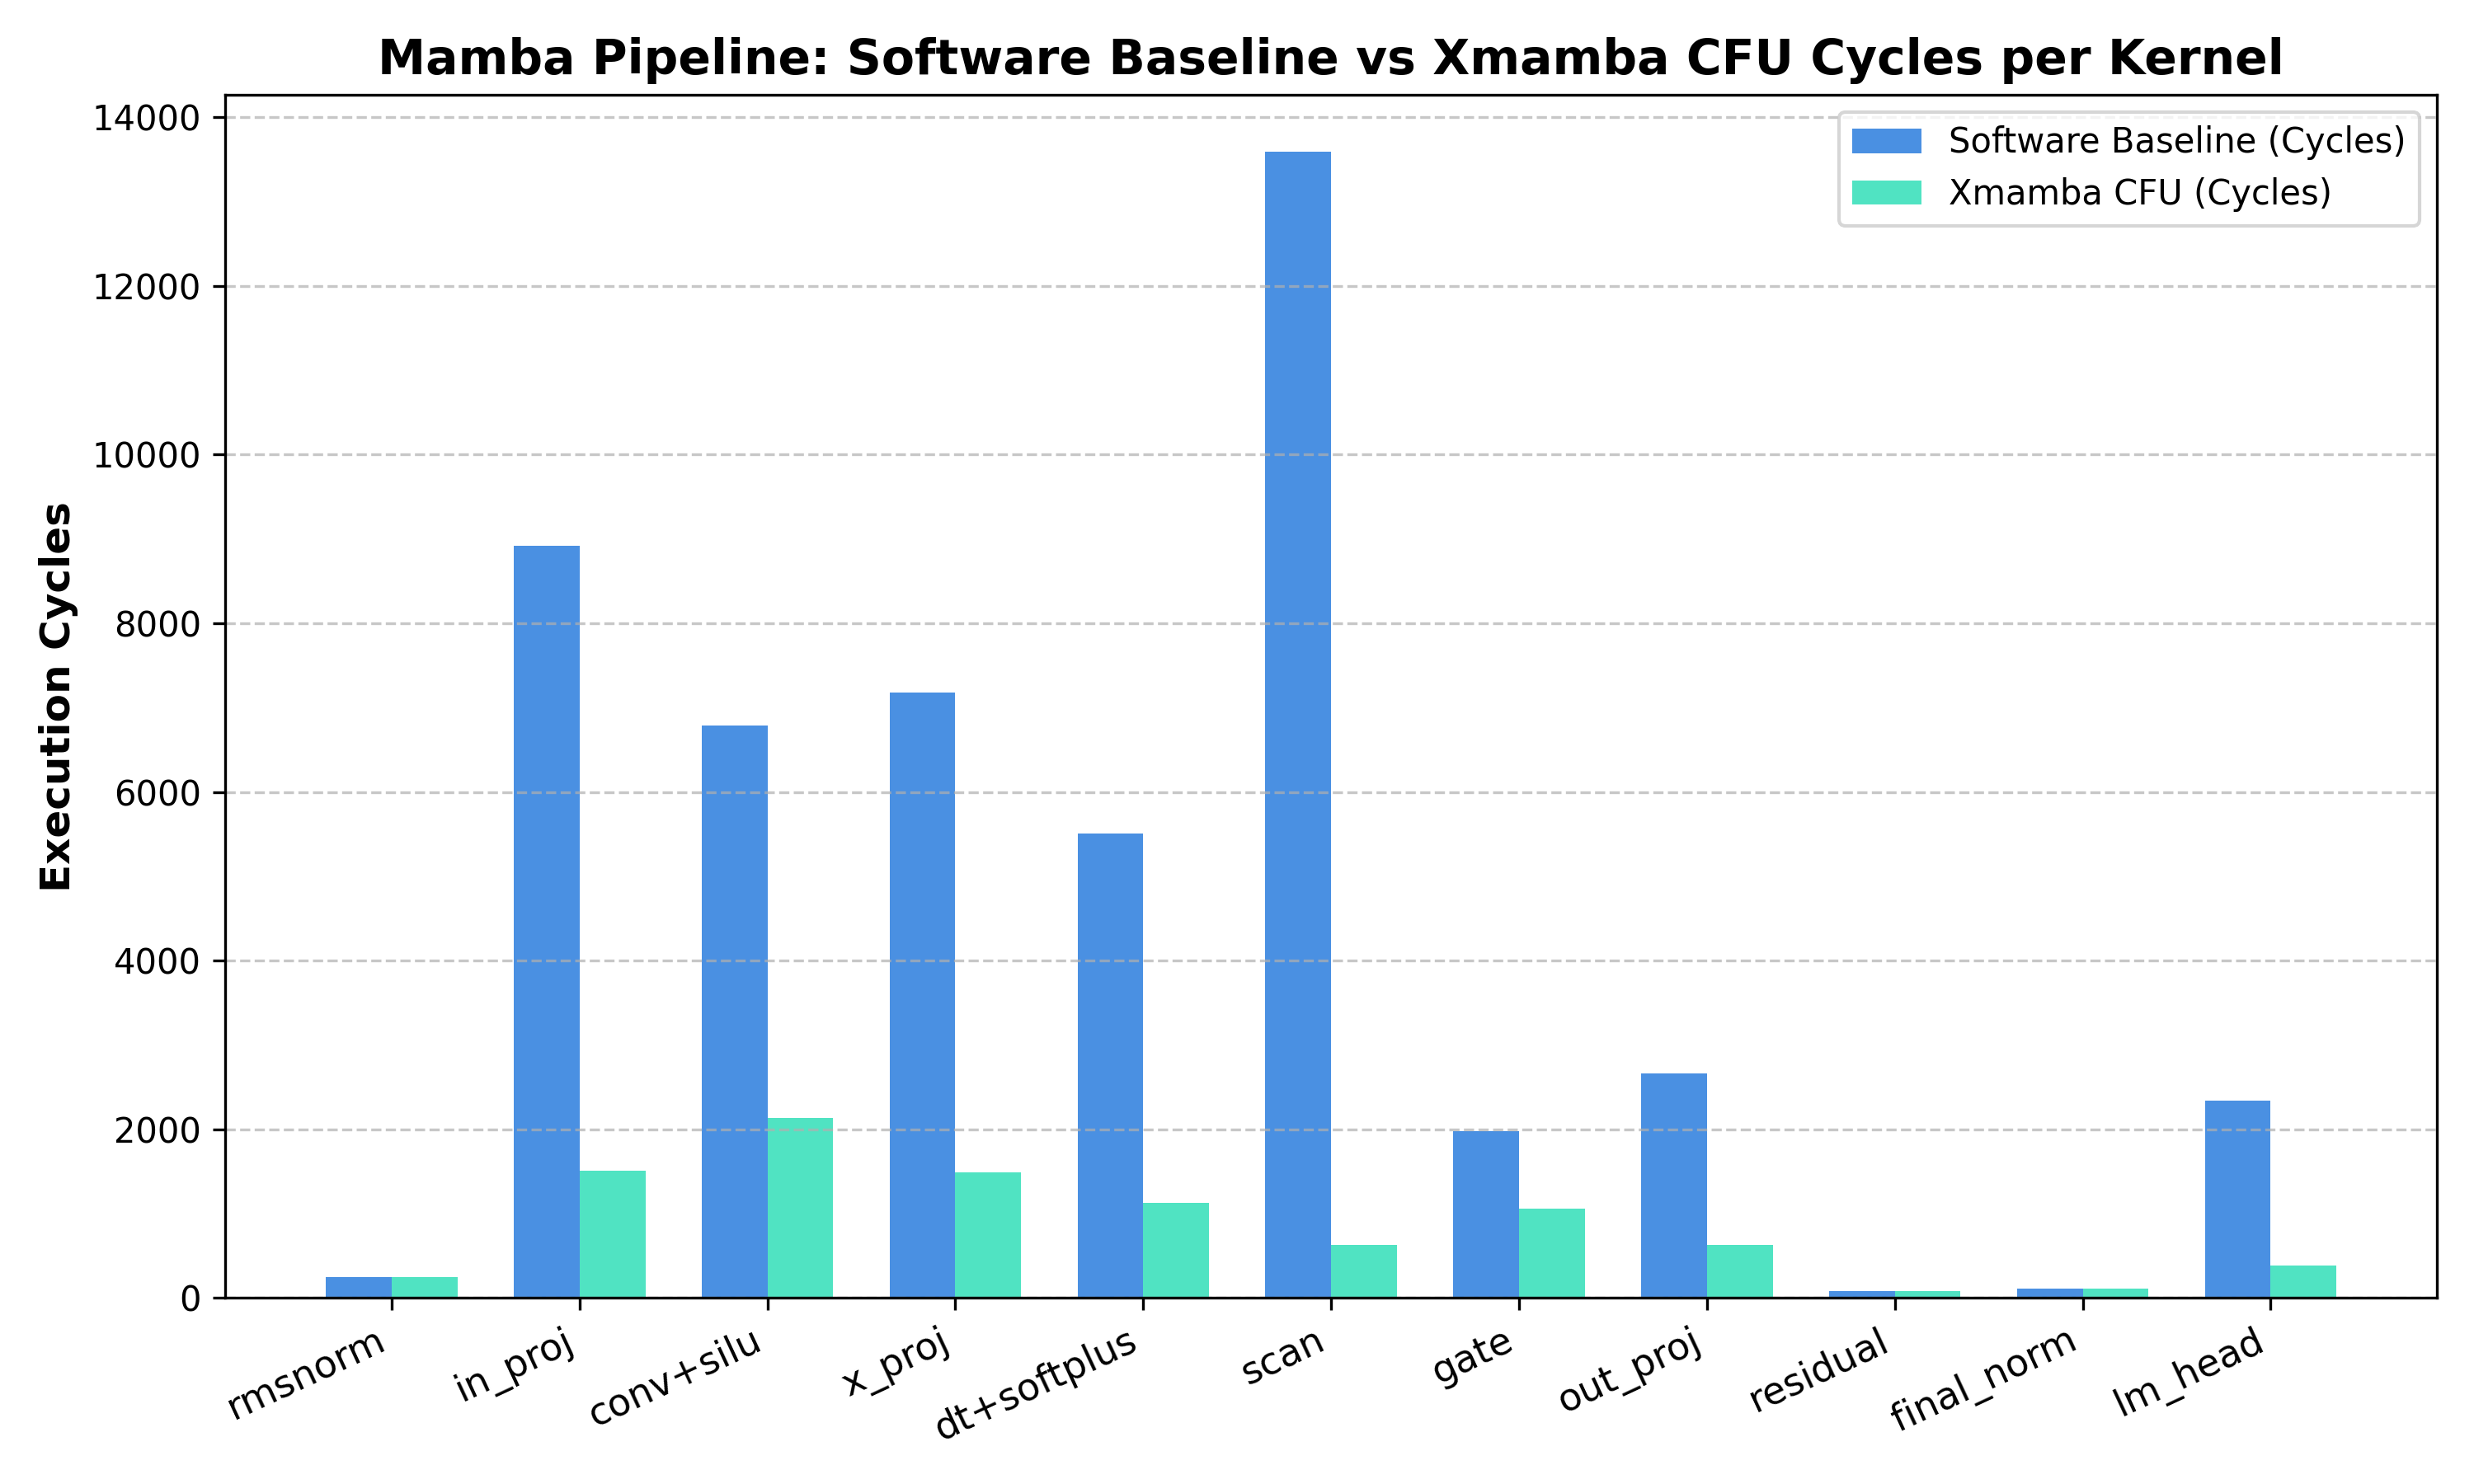
\includegraphics[width=\linewidth]{mamba_kernel_cycles.png}
        \caption{Execution cycles per kernel}
        \label{fig:cycles_chart}
    \end{subfigure}
    \hfill
    \begin{subfigure}[b]{0.48\textwidth}
        \centering
        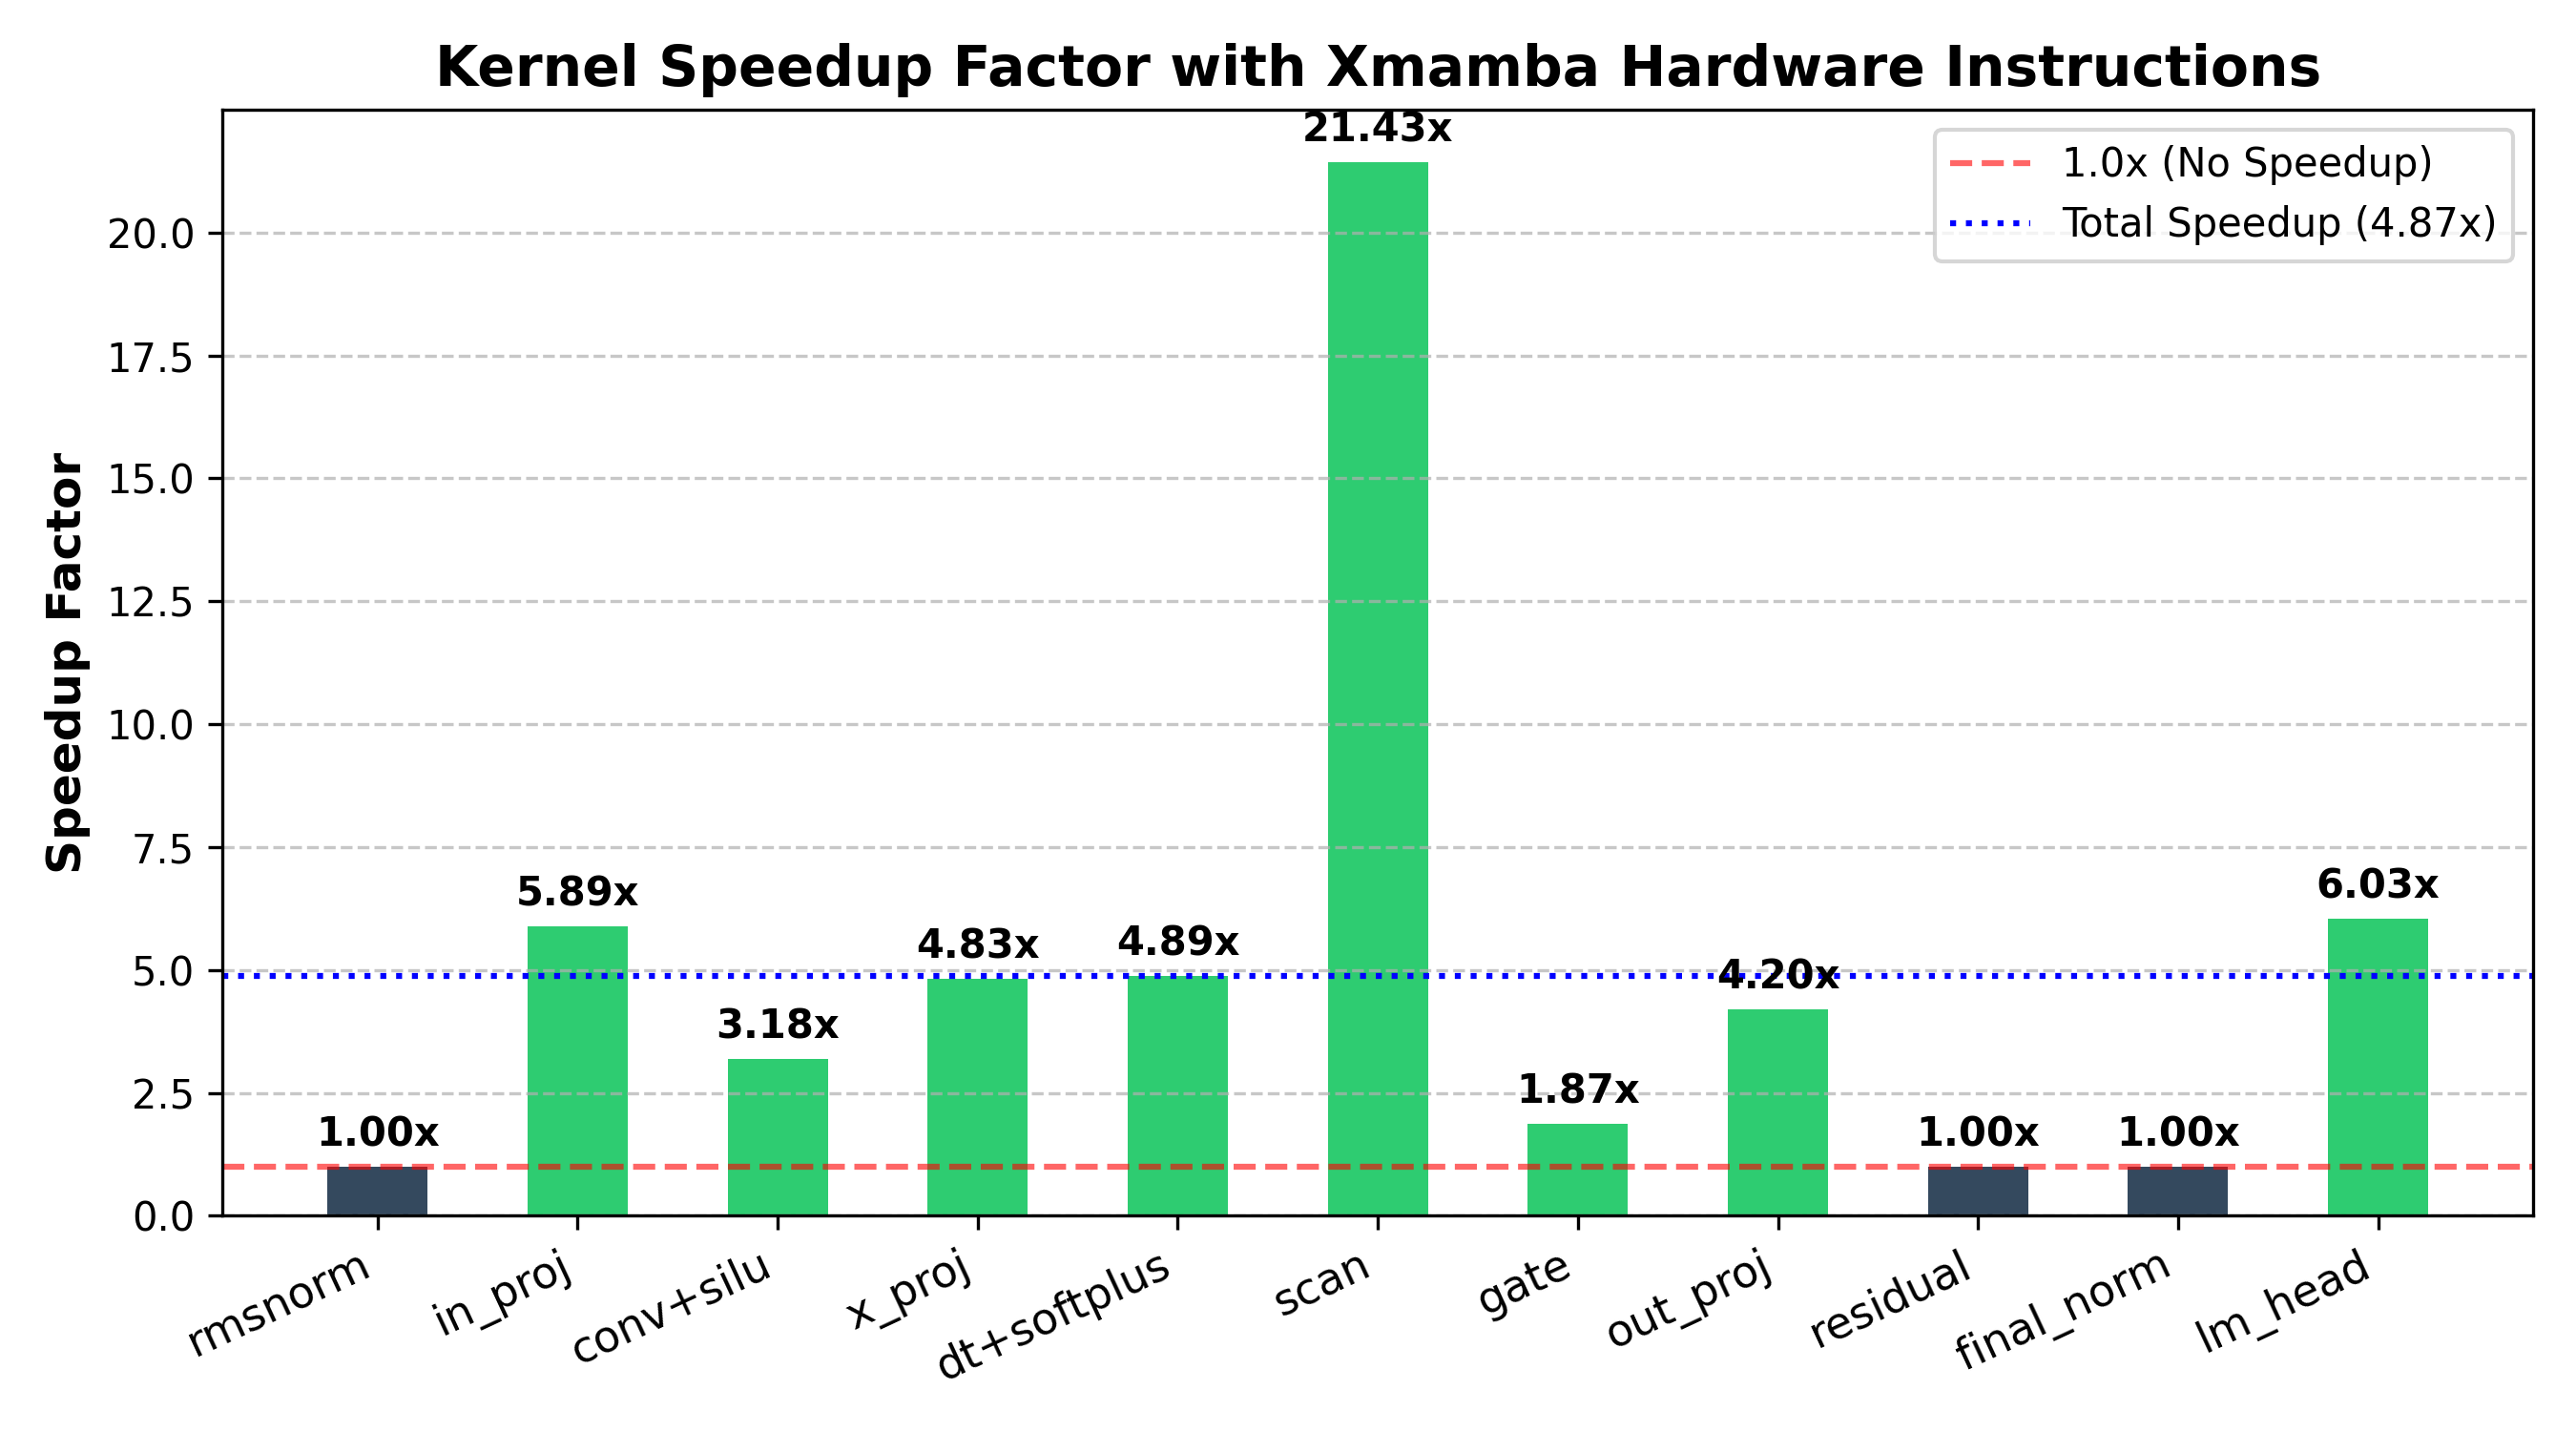
\includegraphics[width=\linewidth]{mamba_kernel_speedup.png}
        \caption{Kernel acceleration factor}
        \label{fig:speedup_chart}
    \end{subfigure}
    \caption[Renode Full-System Performance Profiling]{Full-system Renode SoC performance profiling comparing RV32IM software against Xmamba CFU hardware acceleration.}
    \label{fig:perf_charts}
\end{figure}

The profiling results demonstrate compelling architectural gains:
\begin{itemize}
    \item \textbf{End-to-End Speedup:} Total token execution cycles fall from 50,390 to 10,348, achieving a \textbf{4.87$\times$ end-to-end acceleration}.
    \item \textbf{Selective Scan Engine Acceleration:} The stateful recurrence unit accelerates the scan loop by \textbf{21.43$\times$} ($13,584 \to 634$ cycles), slashing scan instruction fetches by \textbf{95.3\%}.
    \item \textbf{Real-Time Edge Throughput:} At a modest 50 MHz SoC clock, token inference latency drops from $1.008\,\text{ms}$ to \textbf{$206.96\,\mu\text{s}$}, enabling a real-time throughput of \textbf{4,831.9 tokens/second}.
    \item \textbf{Instruction Fetch Reduction:} Total CPU dynamic instruction retirement decreases from 50,389 to 10,347, cutting dynamic instruction fetch energy by \textbf{79.5\%}.
\end{itemize}

\section{Instruction Set Simulator Architectural Ablation (Spike)}
To understand the individual contributions of each custom instruction group, we performed a 4-build architectural ablation on Spike for a larger configuration ($d=256, L=4, 1.82\text{M}$ parameters), as summarized in Table~\ref{tab:spike_ablation}.

\begin{table}[!htbp]
\caption[Four-Build Architectural Ablation on Spike Simulator (d=256, L=4)]{Four-Build Architectural Ablation on Spike Simulator ($d=256, L=4, N=16, 1.82\text{M}$ parameters)}
\label{tab:spike_ablation}
\centering
\begin{tabularx}{\linewidth}{lcccY}
\toprule
\textbf{Build Configuration} & \textbf{Instructions / Token} & \textbf{Speedup} & \textbf{Scan Instructions} & \textbf{Primary Bottleneck} \\
\midrule
1. Software Baseline (RV32IM) & 13,541,056 & 1.00$\times$ & 3,991,110 & ALU dot products \& exp routines \\
2. + MAC Unit (\texttt{mb.mac4, racc}) & 7,629,887 & 1.77$\times$ & 3,991,110 & Unaccelerated scan recurrence \\
3. + Nonlinear Unit (Lookup Tables) & 4,786,727 & 2.83$\times$ & 1,626,336 & Recurrent state register spilling \\
4. Full Xmamba (+ Scan Engine) & \textbf{3,177,371} & \textbf{4.26$\times$} & \textbf{16,980 (235$\times$)} & Register operand bandwidth \\
\bottomrule
\end{tabularx}
\end{table}

This ablation illustrates Amdahl's Law in practice: accelerating only matrix multiplications (+MAC) yields a modest 1.77$\times$ gain because the scan recurrence dominates the remaining execution. Only when the recurrence engine is added does the scan collapse by \textbf{235$\times$} ($3.99\text{M} \to 16.98\text{K}$ instructions), delivering the headline 4.26$\times$ Spike speedup.

\section{Architectural Impact and Memory Hierarchy Benefits}
The measured performance gains validate the architectural decision to modify the RISC-V CPU pipeline rather than deploy a standalone NPU:
\begin{enumerate}
    \item \textbf{Elimination of DMA Setup Tax:} For streaming sensor tokens ($T=16$), setting up DMA control registers and awaiting transfer interrupts would consume hundreds of cycles per token. Tightly coupling the CFU allows single-cycle register operand delivery.
    \item \textbf{On-Chip State Locality:} Retaining recurrent hidden states $h_t \in \mathbb{R}^{8 \times 4}$ inside dedicated CFU BRAM eliminates round-trip memory traffic across the system bus, preserving precious memory bandwidth for weight streaming.
\end{enumerate}

% ----------------------------------------------------------------------
% CHAPTER 7: CONCLUSION AND ROADMAP FOR MAJOR PROJECT -- II
% ----------------------------------------------------------------------
\chapter{CONCLUSION AND ROADMAP FOR MAJOR PROJECT -- II}
\label{Chapter7}
\lhead{Chapter \thechapter. \emph{Conclusion \& Roadmap}}
\rhead{}

\section{Summary of Accomplished Work}
In this Major Project -- I, we conceptualized, architected, and verified \textbf{Xmamba}, a domain-specific custom instruction set extension and tightly-coupled hardware accelerator for fixed-point Mamba state-space inference on embedded RISC-V SoCs. Key accomplishments include:
\begin{itemize}
    \item Designed and trained \textbf{TinyMamba} (636 parameters) on the clinical PhysioNet MIT-BIH Arrhythmia Database, demonstrating 75.26\% validation accuracy and an 80.0\% vs. 33.3\% normal/arrhythmia detection trigger.
    \item Formulated a bit-exact $Q_{16}$ fixed-point quantization recipe achieving \textbf{98.0\% Top-1 agreement} with continuous Float32 models and an MAE of only \textbf{0.0556}.
    \item Specified and ratified the \textbf{10-instruction Xmamba ISA} mapped to RISC-V \texttt{custom-0}, encompassing vector MAC, piecewise-linear nonlinear lookup, and stateful recurrence operations.
    \item Validated \textbf{0.0000 bit-exact RTL equivalence} in Verilog across 6,126 instructions and 880 intermediate tensor stages via cycle-accurate Verilator co-simulation.
    \item Demonstrated a \textbf{4.87$\times$ end-to-end token latency reduction} ($1007.8\,\mu\text{s} \to 206.96\,\mu\text{s}$, or \textbf{4,831.9 tokens/sec}), a \textbf{21.43$\times$ scan speedup}, and a \textbf{79.5\% dynamic instruction reduction} on Renode whole-SoC emulation.
\end{itemize}

\section{Comparison Against Planned Milestones}
Table~\ref{tab:milestone_audit} compares our accomplished progress against the original project plan in \texttt{Milestones.md}. All objectives for Stages 0, 1, 2, and 3 have been completed ahead of schedule.

\begin{table}[!htbp]
\caption[Project Milestone Audit: Planned vs. Accomplished Progress]{Project Milestone Audit: Planned vs. Accomplished Progress}
\label{tab:milestone_audit}
\centering
\begin{tabularx}{\linewidth}{>{\raggedright\arraybackslash\bfseries}p{2.6cm}ccl}
\toprule
\textbf{Milestone Gate} & \textbf{Target Date} & \textbf{Status} & \textbf{Accomplished Evidence} \\
\midrule
Gate 1: Setup \& Onboarding & 08/11/2026 & \textbf{COMPLETED} & Bare-metal Spike runtime, HTIF, crt0.S, hello tests. \\
Gate 2: Reference \& Quantization & 20/11/2026 & \textbf{COMPLETED} & Python/C references, MIT-BIH dataset, 98\% float agreement. \\
Gate 3: ISA Spec v1 Frozen & 11/12/2026 & \textbf{COMPLETED} & 10-instruction spec ratified, \texttt{spec/xmamba-isa.md}. \\
Gate 4: Single Token on SoC Sim & 22/01/2027 & \textbf{COMPLETED} & Renode + Verilator token test passes (\textbf{4.87$\times$ speedup}). \\
Gate 5: Physical FPGA Bring-Up & 12/02/2027 & \textbf{PREPARED} & Out-of-context Vivado script verified; board arrival pending. \\
Final Demo Release & 26/02/2027 & \textbf{ON TRACK} & Final evaluation and hardware demonstrations planned. \\
\bottomrule
\end{tabularx}
\end{table}

\section{Roadmap for Major Project -- II}
The planned roadmap for Major Project -- II (January -- April 2027) encompasses:
\begin{enumerate}
    \item \textbf{Stage 4 (Physical FPGA Implementation):}
    \begin{itemize}
        \item Program the generated LiteX + VexRiscv + Xmamba bitstream onto the physical Digilent Arty A7-100T development board.
        \item Validate USB-UART streaming inference using continuous live ECG playback from laboratory signal generators.
        \item Measure physical board power dissipation and verify timing closure at 50 MHz using the Xilinx Vivado hardware manager.
    \end{itemize}
    \item \textbf{Stage 5 (Evaluation, Freeze \& Dissemination):}
    \begin{itemize}
        \item Conduct extensive multi-hour stability tests across the complete MIT-BIH recording corpus.
        \item Compare physical FPGA throughput against commercial edge platforms (Raspberry Pi Pico, ARM Cortex-M4, GAP9).
        \item Prepare and submit a full research paper to a leading IEEE/ACM venue (e.g. IEEE ISVLSI or ACM GLSVLSI 2027).
    \end{itemize}
\end{enumerate}

% ----------------------------------------------------------------------
% REFERENCES
% ----------------------------------------------------------------------
\clearpage
\begin{thebibliography}{99}
\addcontentsline{toc}{chapter}{References}

\bibitem{gu2023mamba}
A.~Gu and T.~Dao, ``Mamba: Linear-time sequence modeling with selective state spaces,'' \emph{arXiv preprint arXiv:2312.00752}, 2023.

\bibitem{vaswani2017attention}
A.~Vaswani, N.~Shazeer, N.~Parmar, J.~Uszkoreit, L.~Jones, A.~N.~Gomez, \L.~Kaiser, and I.~Polosukhin, ``Attention is all you need,'' in \emph{Advances in Neural Information Processing Systems (NeurIPS)}, vol.~30, 2017, pp. 5998--6008.

\bibitem{gu2021efficiently}
A.~Gu, K.~Goel, and C.~R{\'e}, ``Efficiently modeling long sequences with structured state spaces,'' in \emph{International Conference on Learning Representations (ICLR)}, 2022.

\bibitem{gu2020hippo}
A.~Gu, T.~Dao, S.~Ermon, A.~Rudra, and C.~R{\'e}, ``HiPPO: Recurrent memory with optimal polynomial projections,'' in \emph{Advances in Neural Information Processing Systems (NeurIPS)}, vol.~33, 2020, pp. 1474--1487.

\bibitem{waterman2014risc}
A.~Waterman, Y.~Lee, D.~A.~Patterson, and K.~Asanovi{\'c}, ``The RISC-V instruction set manual, Volume I: User-level ISA, version 2.0,'' Tech. Rep. UCB/EECS-2014-54, EECS Department, UC Berkeley, 2014.

\bibitem{cfu_playground}
T.~Callahan et~al., ``Fast and flexible RISC-V custom instruction exploration with CFU Playground,'' in \emph{Design, Automation \& Test in Europe Conference \& Exhibition (DATE)}, 2023.

\bibitem{vexriscv}
C.~Papon, ``VexRiscv: A modular 32-bit RISC-V processor implemented in SpinalHDL,'' \url{https://github.com/SpinalHDL/VexRiscv}, 2020.

\bibitem{litex}
F.~Bourdeauducq et~al., ``LiteX: An open-source SoC builder and library,'' \url{https://github.com/enjoy-digital/litex}, 2021.

\bibitem{verilator}
W.~Snyder et~al., ``Verilator open-source fast simulator,'' \url{https://www.veripool.org/verilator/}, 2022.

\bibitem{renode}
Antmicro, ``Renode: Open-source software development framework for multi-node embedded systems,'' \url{https://renode.io}, 2023.

\bibitem{mamba_x_2025}
S.~Yoon, H.~Kim, and J.~Lee, ``Mamba-X: Vision Mamba accelerator with systolic scan array and lookup-table function unit,'' in \emph{IEEE/ACM International Conference on Computer-Aided Design (ICCAD)}, 2025.

\bibitem{lightmamba2025}
Y.~Wei, X.~Chen, and Z.~Wang, ``LightMamba: Efficient 4-bit post-training quantization for Mamba state-space models on FPGA,'' in \emph{Design, Automation \& Test in Europe Conference (DATE)}, 2025.

\bibitem{marca2024}
L.~Zhang et~al., ``MARCA: A reconfigurable Mamba accelerator with unified processing elements,'' in \emph{IEEE/ACM International Conference on Computer-Aided Design (ICCAD)}, 2024.

\bibitem{femba2026}
M.~Gao et~al., ``FEMBA on the Edge: Deploying quantized state-space models on ultra-low-power RISC-V microcontrollers,'' in \emph{IEEE Transactions on Biomedical Circuits and Systems}, 2026.

\bibitem{goldberger2000physiobank}
A.~L.~Goldberger et~al., ``PhysioBank, PhysioToolkit, and PhysioNet: Components of a new research resource for complex physiologic signals,'' \emph{Circulation}, vol. 101, no.~23, pp. e215--e220, 2000.

\bibitem{moodie1983mitbih}
G.~B.~Moody and R.~G.~Mark, ``The impact of the MIT-BIH Arrhythmia Database,'' \emph{IEEE Engineering in Medicine and Biology Magazine}, vol.~20, no.~3, pp. 45--50, 2001.

\end{thebibliography}

\end{document}
